% ============================================================================
% Livrable 2 - Projet Cloud Healthcare Unit (CHU)
% Rapport d'implementation physique et d'evaluation de performance
% ============================================================================
\documentclass[11pt,a4paper]{article}

\usepackage[utf8]{inputenc}
\usepackage[T1]{fontenc}
\usepackage{lmodern}
\usepackage[french]{babel}
\usepackage[a4paper,margin=2.2cm,top=2.5cm,bottom=2.5cm]{geometry}
\sloppy
\emergencystretch=3em
\usepackage{graphicx}
\usepackage{booktabs}
\usepackage{longtable}
\usepackage{array}
\usepackage[table]{xcolor}
\usepackage[hidelinks]{hyperref}
\usepackage{caption}
\usepackage{float}
\usepackage{enumitem}
\usepackage{microtype}
\usepackage{fancyhdr}
\usepackage{titlesec}
\usepackage{listings}
\usepackage{tikz}
\usetikzlibrary{positioning,arrows.meta}
\usepackage{pgfplots}
\pgfplotsset{compat=1.18}

% --- blocs code en \small ----------------------------------------------------
\lstset{
  basicstyle=\ttfamily\small,
  columns=flexible, keepspaces=true, frame=single, framerule=0.4pt,
  breaklines=true, showstringspaces=false, tabsize=2,
}
\lstnewenvironment{sqlcode}{\shorthandoff{;:!?}}{\shorthandon{;:!?}}

% --- tableaux generes depuis les rapports de resultats du projet ------------
% Tables generees depuis les CSV reels du projet (ne pas editer a la main)

\newcommand{\rowsdqvolumes}{%
S1.PostgreSQL (dump DATA2023) & Patient & 100000 &  \\
S1.PostgreSQL (dump DATA2023) & Consultation & 1027157 & 2015-06-20 -> 2023-03-31 \\
S1.PostgreSQL (dump DATA2023) & Diagnostic & 15490 &  \\
S1.PostgreSQL (dump DATA2023) & Professionnel\_de\_sante & 1048575 &  \\
S1.PostgreSQL (dump DATA2023) & Specialites & 93 &  \\
S1.PostgreSQL (dump DATA2023) & Salle & 201735 &  \\
S1.PostgreSQL (dump DATA2023) & Adher & 96671 &  \\
S1.PostgreSQL (dump DATA2023) & Mutuelle & 254 &  \\
S1.PostgreSQL (dump DATA2023) & Prescription & 1003845 &  \\
S1.PostgreSQL (dump DATA2023) & Medicaments & 15455 &  \\
S1.PostgreSQL (dump DATA2023) & Laboratoire & 677 &  \\
S1.PostgreSQL (dump DATA2023) & AAAA & 82216 &  \\
S1.PostgreSQL (dump DATA2023) & date & 82216 &  \\
S2.Hospitalisations.csv & Hospitalisations.csv & 2479 & 2015-06-21 00:00:00 -> 2021-06-19 00:00:00 \\
S3/ESATIS & satisfaction\_2019.csv & 1152 & 2019 \\
S3/ESATIS & satisfaction\_2020.csv & 1143 & 2020 \\
S4.INSEE & deces.csv & 25088208 & 1882-10-01 -> 2020-03-30 \\
Referentiel FINESS & etablissement\_sante.csv & 416665 &  \\
Referentiel FINESS & professionnel\_sante.csv & 1048575 &  \\
Referentiel FINESS & activite\allowbreak\_professionnel\allowbreak\_sante.csv & 1823588 &  \\
}%

\newcommand{\rowsdqcompletude}{%
Hospitalisations & Num\_Hospitalisation & 2479 & 2479 & 100 \\
Hospitalisations & Id\_patient & 2479 & 2479 & 100 \\
Hospitalisations & identifiant\_organisation & 2479 & 2479 & 100 \\
Hospitalisations & Code\_diagnostic & 2479 & 2479 & 100 \\
Hospitalisations & Date\_Entree & 2479 & 2479 & 100 \\
Hospitalisations & Jour\_Hospitalisation & 2479 & 2479 & 100 \\
S1\_Patient & Sexe & 100000 & 100000 & 100 \\
S1\_Patient & Date\_naissance & 100000 & 100000 & 100 \\
S1\_Patient & Age & 100000 & 100000 & 100 \\
S1\_Patient & Num\_Secu & 100000 & 100000 & 100 \\
S1\_Consultation & Date & 1027157 & 1027157 & 100 \\
S1\_Consultation & Code\_diag & 1027157 & 1027157 & 100 \\
S1\_Consultation & Id\_prof\_sante & 1027157 & 1027157 & 100 \\
deces & sexe & 25088208 & 25088208 & 100 \\
deces & date\_deces & 25088208 & 25088208 & 100 \\
deces & date\_naissance & 25088208 & 25087658 & 100 \\
deces & code\_lieu\_deces & 25088208 & 25077274 & 99,96 \\
etablissement & finess\_site & 416665 & 200 & 0,05 \\
etablissement & finess\_etablissement\_juridique & 416665 & 57692 & 13,85 \\
etablissement & identifiant\_organisation & 416665 & 416665 & 100 \\
etablissement & code\_commune & 416665 & 277860 & 66,69 \\
professionnel\_sante & identifiant & 1048575 & 1048575 & 100 \\
satisfaction\_2019 & score\_all\_rea\_ajust & 1152 & 858 & 74,48 \\
satisfaction\_2020 & score\_all\_rea\_ajust & 1143 & 832 & 72,79 \\
satisfaction\_2019 & score\_all\_rea\_ajust normalise (non NULL) & 1152 & 858 & 74,48 \\
satisfaction\_2020 & score\_all\_rea\_ajust normalise (non NULL) & 1143 & 832 & 72,79 \\
}%

\newcommand{\rowsdqcompletudefaits}{%
gold.f\_mesures & annee\_mois & 1030402 & 1030402 & 100 \\
gold.f\_mesures & id\_etablissement & 1030402 & 1030402 & 100 \\
gold.f\_mesures & id\_patient & 1030402 & 1030402 & 100 \\
gold.f\_mesures & id\_localisation & 1030402 & 1030402 & 100 \\
gold.f\_mesures & nbre\_consultation & 1030402 & 1030402 & 100 \\
gold.f\_mesures & nbre\_hospitalisation & 1030402 & 1030402 & 100 \\
gold.f\_mesures & total\_satisfaction & 1030402 & 33 & 0 \\
gold.f\_mesures & nbre\_deces & 1030402 & 1030402 & 100 \\
gold.f\_mesures & region & 1030402 & 1030402 & 100 \\
gold.f\_hospitalisation & id\_hospitalisation & 2479 & 2479 & 100 \\
gold.f\_hospitalisation & id\_temps & 2479 & 2479 & 100 \\
gold.f\_hospitalisation & id\_patient & 2479 & 2479 & 100 \\
gold.f\_hospitalisation & id\_diagnostic & 2479 & 2479 & 100 \\
gold.f\_hospitalisation & id\_etablissement & 2479 & 2479 & 100 \\
gold.f\_hospitalisation & id\_localisation & 2479 & 2479 & 100 \\
gold.f\_hospitalisation & duree\_jours & 2479 & 2479 & 100 \\
gold.f\_satisfaction & finess & 1960 & 1960 & 100 \\
gold.f\_satisfaction & region & 1960 & 1960 & 100 \\
gold.f\_satisfaction & score\_satisfaction & 1960 & 1523 & 77,7 \\
gold.f\_satisfaction & nb\_repondants & 1960 & 1523 & 77,7 \\
gold.f\_satisfaction & nb\_sites & 1960 & 1960 & 100 \\
silver.f\_consultation\_detail & id\_consultation & 1027157 & 1027157 & 100 \\
silver.f\_consultation\_detail & id\_temps & 1027157 & 1027157 & 100 \\
silver.f\_consultation\_detail & id\_patient & 1027157 & 1027157 & 100 \\
silver.f\_consultation\_detail & id\_diagnostic & 1027157 & 1027157 & 100 \\
silver.f\_consultation\_detail & id\_professionnel & 1027157 & 1027157 & 100 \\
silver.f\_consultation\_detail & id\_etablissement & 1027157 & 1027157 & 100 \\
silver.f\_consultation\_detail & id\_localisation & 1027157 & 1027157 & 100 \\
}%

\newcommand{\rowsdqvalidite}{%
deces & date\_deces format ISO AAA-MM-JJ & 25088208 & 646 & 0,0026 \\
deces & date\_naissance format ISO & 25088208 & 89898 & 0,3583 \\
deces & sexe dans \{1,2\} & 25088208 & 0 & 0 \\
Hospitalisations & Date\_Entree format JJ/MM/AAAA & 2479 & 0 & 0 \\
Hospitalisations & Code\_diagnostic format CIM-10 & 2479 & 368 & 14,8447 \\
S1\_Patient & Sexe dans \{male,female\} & 100000 & 0 & 0 \\
S1\_Patient & Date\_naissance format M/J/AAAA & 100000 & 0 & 0 \\
etablissement & finess\_site 9 caracteres (non vides) & 200 & 0 & 0 \\
satisfaction\_2019 & finess 9 caracteres & 1152 & 7 & 0,6076 \\
satisfaction\_2019 & score\_all\_rea\_ajust decimal (virgule) & 1152 & 0 & 0 \\
satisfaction\_2020 & finess 9 caracteres & 1143 & 0 & 0 \\
satisfaction\_2020 & score\_all\_rea\_ajust decimal (virgule) & 1143 & 0 & 0 \\
}%

\newcommand{\rowsdqdoublons}{%
Hospitalisations & Num\_Hospitalisation & 2479 & 0 & 0 \\
S1\_Consultation & Num\_consultation & 1027157 & 0 & 0 \\
S1\_Patient & Id\_patient & 100000 & 0 & 0 \\
etablissement (finess\_site non vide) & finess\_site & 200 & 0 & 0 \\
etablissement (toutes cles) & identifiant\_organisation & 416665 & 0 & 0 \\
satisfaction\_2019 & finess (grain brut) & 1152 & 166 & 14,4097 \\
satisfaction\_2019 & finess + finess\_geo (grain reel) & 1152 & 0 & 0 \\
satisfaction\_2020 & finess + finess\_geo (grain reel) & 1143 & 0 & 0 \\
deces & cle complete (nom, prenom, date\_naissance, date\_deces, lieu, acte) & 25088208 & 174794 & 0,6967 \\
}%

\newcommand{\rowsdqdoublonsfaits}{%
f\_consultation\_detail (fait int\'egr\'e, Silver) & id\_consultation (grain 1 consultation) & 1027157 & 0 & 0 \\
f\_hospitalisation (fait int\'egr\'e, Gold) & id\_hospitalisation (grain 1 hospitalisation) & 2479 & 0 & 0 \\
f\_satisfaction (fait int\'egr\'e, Gold) & annee + finess (grain etab. juridique x annee) & 1960 & 0 & 0 \\
f\_mesures (fait consolid\'e, Gold) & annee\_mois + id\_etablissement + id\_patient + sexe + tranche\_age + id\_localisation + region & 1030402 & 0 & 0 \\
}%

\newcommand{\rowsdqreferentiel}{%
Hospitalisations.identifiant\_organisation -> etab.identifiant\_organisation & 2479 & 2479 & 100 \\
Hospitalisations.identifiant\_organisation -> etab.finess\_etablissement\_juridique & 2479 & 0 & 0 \\
Hospitalisations.identifiant\_organisation -> etab.finess\_site & 2479 & 0 & 0 \\
Hospitalisations.Id\_patient -> S1.Patient.Id\_patient & 2479 & 2479 & 100 \\
Hospitalisations.Code\_diagnostic -> S1.Diagnostic.Code\_diag & 2479 & 2479 & 100 \\
satisfaction\_2019.finess -> etab.finess\_etablissement\_juridique & 1152 & 575 & 49,91 \\
satisfaction\_2019.finess\_geo -> etab.finess\_site & 1152 & 0 & 0 \\
satisfaction\_2020.finess -> etab.finess\_etablissement\_juridique & 1143 & 580 & 50,74 \\
satisfaction\_2020.finess\_geo -> etab.finess\_site & 1143 & 0 & 0 \\
activite.identifiant -> pro\_referentiel.identifiant & 1823588 & 1042874 & 57,19 \\
activite.identifiant\_organisation -> etab.identifiant\_organisation & 1823588 & 1464774 & 80,32 \\
S1.Consultation.Id\_prof\_sante -> pro\_referentiel.identifiant & 1027157 & 1027157 & 100 \\
S1.Consultation.Id\_prof\_sante -> activite.identifiant & 1027157 & 738190 & 71,87 \\
satisfaction\_2019.finess -> etab.identifiant\_organisation & 1152 & 0 & 0 \\
satisfaction\_2020.finess -> etab.identifiant\_organisation & 1143 & 0 & 0 \\
etablissement.code\_commune -> departement (regle INSEE, non vides) & 277860 & 277127 & 99,74 \\
deces.code\_lieu\_deces -> departement (regle INSEE, non vides) & 25077274 & 24876383 & 99,2 \\
satisfaction\_2019.region brute -> region normalisee (mapping) & 1152 & 1140 & 98,96 \\
satisfaction\_2020.region brute -> region normalisee (mapping) & 1143 & 1130 & 98,86 \\
satisfaction\_2019.region normalisee -> referentiel region & 1140 & 1140 & 100 \\
satisfaction\_2020.region normalisee -> referentiel region & 1130 & 1130 & 100 \\
satisfaction\_2020: concordance region ESATIS vs region etab (via finess juridique) & 8308 & 8027 & 96,62 \\
}%

\newcommand{\rowsdqintegritefk}{%
f\_mesures.id\_etablissement -> d\_etablissement.id\_etablissement & 658525 & 658525 & 100 \\
f\_mesures.id\_patient -> d\_patient.id\_patient & 1022064 & 1022064 & 100 \\
f\_mesures.id\_localisation -> d\_localisation.id\_localisation & 665288 & 665288 & 100 \\
f\_mesures.id\_temps -> d\_temps.id\_temps & 1022064 & 1022064 & 100 \\
f\_consultation\_detail.id\_patient -> d\_patient.id\_patient & 1027157 & 1027157 & 100 \\
f\_consultation\_detail.id\_etablissement -> d\_etablissement.id\_etablissement & 1027157 & 656063 & 63,87 \\
f\_consultation\_detail.id\_diagnostic -> d\_diagnostic.id\_diagnostic & 1027157 & 1027157 & 100 \\
f\_consultation\_detail.id\_professionnel -> d\_professionnel.identifiant & 1027157 & 1027157 & 100 \\
f\_consultation\_detail.id\_localisation -> d\_localisation.id\_localisation & 654605 & 654605 & 100 \\
f\_hospitalisation.id\_patient -> d\_patient.id\_patient & 2479 & 2479 & 100 \\
f\_hospitalisation.id\_diagnostic -> d\_diagnostic.id\_diagnostic & 2479 & 2479 & 100 \\
f\_hospitalisation.id\_etablissement -> d\_etablissement.id\_etablissement & 2479 & 2479 & 100 \\
f\_hospitalisation.id\_localisation -> d\_localisation.id\_localisation & 2479 & 2479 & 100 \\
}%

\newcommand{\rowsdqtemporel}{%
Hospitalisations & Date\_Entree dans [2015,2023] & 2479 & 2479 & 100 & 2015-06-21 00:00:00 -> 2021-06-19 00:00:00 \\
S1\_Consultation & Date dans [2015,2023] & 1027157 & 1027157 & 100 & 2015-06-20 -> 2023-03-31 \\
deces & date\_deces >= date\_naissance & 25088208 & 24997051 & 99,64 & 1882-10-01 -> 2020-03-30 \\
S1\_Patient & coherence Age vs date\_naissance (|ecart|<=2 ans) & 100000 & 45998 & 46 & age 0..100 observe \\
satisfaction\_2019 & score\_all\_rea\_ajust dans [0,100] & 1152 & 858 & 74,48 & scores 0-100 \\
satisfaction\_2020 & score\_all\_rea\_ajust dans [0,100] & 1143 & 832 & 72,79 & scores 0-100 \\
}%

\newcommand{\rowsbench}{%
q01 & 39 & 99 & 30 & 1,3 & 20050266 & 13619309 & 1,5 \\
q02 & 16,5 & 30 & 14,5 & 1,14 & 6159571 & 2529991 & 2,4 \\
q03 & 5,5 & 74 & 17,5 & 0,31 & 9542613 & 7678170 & 1,2 \\
q04 & 6 & 13 & 8 & 0,75 & 451286 & 596575 & 0,8 \\
q05 & 3 & 75 & 16,5 & 0,18 & 9542613 & 7678170 & 1,2 \\
q06 & 47 & 68,5 & 58,5 & 0,8 & 23788200 & 19652297 & 1,2 \\
q07 & 7 & 59,5 & 6 & 1,17 & 328312 & 24037 & 13,7 \\
q08 & 2,5 & 14 & 5,5 & 0,45 & 23231 & 26883 & 0,9 \\
q09 & 9 & 81,5 & 14 & 0,64 & 9542613 & 4429225 & 2,2 \\
q10 & 29 & 125 & 32 & 0,91 & 21292573 & 14374510 & 1,5 \\
}%

\newcommand{\rowsbenchmo}{%
q01 & 39 & 99 & 30 & 1,3 & 20,0503 & 13,6193 & 1,5 \\
q02 & 16,5 & 30 & 14,5 & 1,14 & 6,15957 & 2,52999 & 2,4 \\
q03 & 5,5 & 74 & 17,5 & 0,31 & 9,54261 & 7,67817 & 1,2 \\
q04 & 6 & 13 & 8 & 0,75 & 0,451286 & 0,596575 & 0,8 \\
q05 & 3 & 75 & 16,5 & 0,18 & 9,54261 & 7,67817 & 1,2 \\
q06 & 47 & 68,5 & 58,5 & 0,8 & 23,7882 & 19,6523 & 1,2 \\
q07 & 7 & 59,5 & 6 & 1,17 & 0,328312 & 0,024037 & 13,7 \\
q08 & 2,5 & 14 & 5,5 & 0,45 & 0,023231 & 0,026883 & 0,9 \\
q09 & 9 & 81,5 & 14 & 0,64 & 9,54261 & 4,42922 & 2,2 \\
q10 & 29 & 125 & 32 & 0,91 & 21,2926 & 14,3745 & 1,5 \\
}%

\newcommand{\rowstrinoraw}{%
q01\_consult\_etab\_2019 & 2277 & 19 \\
q01\_consult\_etab\_2019 & 1714 & 19 \\
q01\_consult\_etab\_2019 & 1504 & 19 \\
q02\_consult\_diag\_2019\_2021 & 1432 & 9 \\
q02\_consult\_diag\_2019\_2021 & 1243 & 9 \\
q02\_consult\_diag\_2019\_2021 & 1143 & 9 \\
q03\_taux\_hosp\_periode & 1472 & 6 \\
q03\_taux\_hosp\_periode & 1389 & 6 \\
q03\_taux\_hosp\_periode & 1413 & 6 \\
q04\_hosp\_diag & 1200 & 9 \\
q04\_hosp\_diag & 1135 & 9 \\
q04\_hosp\_diag & 1113 & 9 \\
q05\_hosp\_sexe\_age & 1522 & 11 \\
q05\_hosp\_sexe\_age & 1340 & 11 \\
q05\_hosp\_sexe\_age & 1438 & 11 \\
q06\_consult\_prof\_2020 & 2005 & 9 \\
q06\_consult\_prof\_2020 & 1823 & 9 \\
q06\_consult\_prof\_2020 & 1719 & 9 \\
q07\_deces\_region\_2019 & 1371 & 18 \\
q07\_deces\_region\_2019 & 1126 & 18 \\
q07\_deces\_region\_2019 & 1176 & 18 \\
q08\_satisfaction\_region\_2020 & 1228 & 15 \\
q08\_satisfaction\_region\_2020 & 1161 & 15 \\
q08\_satisfaction\_region\_2020 & 1126 & 15 \\
q09\_vue\_taux\_mensuel & 2225 & 50 \\
q09\_vue\_taux\_mensuel & 1609 & 50 \\
q09\_vue\_taux\_mensuel & 1816 & 50 \\
q10\_etoile\_complete & 1742 & 19 \\
q10\_etoile\_complete & 1655 & 19 \\
q10\_etoile\_complete & 1531 & 19 \\
}%

\newcommand{\rowstrino}{%
q01\_consult\_etab\_2019 & 1714 & 1504 & 2277 & 19 \\
q02\_consult\_diag\_2019\_2021 & 1243 & 1143 & 1432 & 9 \\
q03\_taux\_hosp\_periode & 1413 & 1389 & 1472 & 6 \\
q04\_hosp\_diag & 1135 & 1113 & 1200 & 9 \\
q05\_hosp\_sexe\_age & 1438 & 1340 & 1522 & 11 \\
q06\_consult\_prof\_2020 & 1823 & 1719 & 2005 & 9 \\
q07\_deces\_region\_2019 & 1176 & 1126 & 1371 & 18 \\
q08\_satisfaction\_region\_2020 & 1161 & 1126 & 1228 & 15 \\
q09\_vue\_taux\_mensuel & 1816 & 1609 & 2225 & 50 \\
q10\_etoile\_complete & 1655 & 1531 & 1742 & 19 \\
}%


\definecolor{starblue}{RGB}{187,214,240}
\definecolor{factred}{RGB}{240,190,190}
\definecolor{silvergreen}{RGB}{200,230,200}

\captionsetup{font=small,labelfont=bf}
\pagestyle{fancy}
\fancyhf{}
\fancyhead[L]{\small Livrable 2 -- Cloud Healthcare Unit (CHU)}
\fancyhead[R]{\small Implementation physique \& evaluation de performance}
\fancyfoot[C]{\thepage}
\renewcommand{\headrulewidth}{0.4pt}

\titleformat{\section}{\Large\bfseries}{\thesection}{1em}{}
\titleformat{\subsection}{\large\bfseries}{\thesubsection}{1em}{}

\begin{document}

% ============================ PAGE DE TITRE =================================
\begin{titlepage}
\centering
\vspace*{2cm}
{\LARGE \textbf{Projet Cloud Healthcare Unit (CHU)}\\[0.4cm]}
{\Large Entrepot de donnees decisionnel hospitalier\\[1.2cm]}
{\Huge \textbf{Livrable 2}\\[0.3cm]}
{\LARGE Implementation physique et evaluation de performance\\[1.5cm]}
\rule{0.7\textwidth}{0.5pt}\\[1.2cm]
{\large
\begin{tabular}{rl}
\textbf{Auteurs} & Tony Fages, Martin Caparros, David d'Almeida \\
\textbf{Date} & 29 octobre 2026 \\
\textbf{Format} & Rapport + archive ZIP (format demande par le sujet) \\
\textbf{Stack} & MinIO (lake) + Hive Metastore + Spark + Airflow \\
 & + Trino + Superset (17 services conteneurises) \\
\end{tabular}
}\\[1.5cm]
\rule{0.7\textwidth}{0.5pt}\\[0.8cm]
{\small
Ce rapport couvre le \textbf{Livrable 2} du sujet : DDL/DML commentes,
partitionnement et indexation justifies par le moteur, rapport de qualite des
donnees integrees, jeu de requetes de benchmark (10 requetes) et evaluation de
performance avant/apres partitionnement.
}
\vfill
{\footnotesize Tous les chiffres cites proviennent des mesures realisees sur la
plateforme et des rapports de controles qualite du projet.}
\end{titlepage}

\tableofcontents
\newpage

% ============================ 2. ARCHITECTURE ===============================
\section{Architecture de la plateforme}

\begin{figure}[H]\centering
\caption{Architecture de bout en bout -- 17 services conteneurises}
\resizebox{\textwidth}{!}{%
\begin{tikzpicture}[
  box/.style={draw, rounded corners=2pt, minimum width=4.6cm, minimum height=0.95cm, align=center, font=\small},
  arr/.style={-{Stealth[length=2.5mm]}, thick}
]
\node[box, fill=gray!15] (src) at (0,6.2) {Sources : S1 PostgreSQL + S2/S3/S4\\(CSV, ESATIS, INSEE/FINESS)};
\node[box, fill=orange!20] (ing) at (0,4.4) {Ingestion $\rightarrow$ zone \texttt{raw/}};
\node[box, fill=blue!15] (minio) at (0,2.4) {\textbf{MinIO} -- data lake\\\texttt{raw/ silver/ gold/} (Parquet)};
\node[box, fill=purple!15] (meta) at (0,0.4) {\textbf{Hive Metastore} + HiveServer2\\(catalogue : tables externes, partitions)};
\node[box, fill=green!20] (spark) at (-6.4,2.4) {\textbf{Apache Spark}\\ETL/ELT $\rightarrow$ Silver/Gold};
\node[box, fill=yellow!25] (air) at (-6.4,4.4) {\textbf{Apache Airflow}\\DAGs init + daily};
\node[box, fill=red!15] (trino) at (6.4,2.4) {\textbf{Trino}\\requetage (connecteur Hive)};
\node[box, fill=red!25] (sup) at (6.4,0.4) {\textbf{Apache Superset}\\8 tableaux de bord};
\draw[arr] (src) -- (ing);
\draw[arr] (ing) -- (minio);
\draw[arr] (spark) -- (minio);
\draw[arr] (air) -- (spark);
\draw[arr] (minio) -- (meta);
\draw[arr] (meta) -- (trino);
\draw[arr] (minio) -- (trino);
\draw[arr] (trino) -- (sup);
\end{tikzpicture}%
}
\end{figure}

La chaine de production a ete executee de bout en bout : DAG d'initialisation
(5/5 taches en succes) puis DAG journalier (8/8 taches en succes) ; les volumes
ont ete re-verifies dans Trino (\S3.3) et des captures d'ecran des interfaces de
la plateforme sont presentees en \S3.4.

% ============================ 3. MODELE PHYSIQUE ============================
\section{Modele physique : schema en etoile}

\subsection{Schema en etoile}
Le modele du Livrable 1 est implemente en couche \textbf{Gold} (decisionnel) sur
le data lake, avec une couche \textbf{Silver} pour le fait de detail des
consultations. \textbf{13 tables externes (12 Gold + 1 Silver)}, toutes en
\texttt{CREATE EXTERNAL TABLE ... STORED AS PARQUET LOCATION 's3a://lake/...'}
(les donnees appartiennent au lake ; un \texttt{DROP TABLE} ne supprime jamais
les donnees). Les cles de substitution (surrogate keys) sont presentes dans les
dimensions : \texttt{id\_temps} (AAAAMMJJ), \texttt{id\_patient},
\texttt{id\_etablissement} (\texttt{row\_number}), \texttt{id\_localisation}
(code departement), \texttt{id\_diagnostic} (\texttt{row\_number}),
\texttt{identifiant} (professionnel).

\begin{figure}[H]\centering
\caption{Schema en etoile deploye (couches Gold/Silver)}
\resizebox{\textwidth}{!}{%
\begin{tikzpicture}[
  dim/.style={draw, fill=starblue, minimum width=3.1cm, minimum height=0.85cm, align=center, font=\small},
  fact/.style={draw, fill=factred, minimum width=5.2cm, minimum height=1.7cm, align=center, font=\small},
  sil/.style={draw, fill=silvergreen, minimum width=4.4cm, minimum height=1.0cm, align=center, font=\small},
  arr/.style={-{Stealth[length=2mm]}, thick}
]
\node[fact] (fm) {\textbf{f\_mesures} (Gold)\\grain : annee\_mois $\times$ etab $\times$ patient $\times$ sexe\\$\times$ tranche\_age $\times$ loc $\times$ region\\4 mesures : consultation, hospitalisation,\\satisfaction, deces};
\node[dim, above=1.7cm of fm] (dt) {\textbf{d\_temps}\\jour 2015--2030, id\_temps};
\node[dim, left=1.6cm of fm] (dp) {\textbf{d\_patient}\\100 000, id\_patient\\part. sexe, tranche\_age\_ref};
\node[dim, right=1.6cm of fm] (de) {\textbf{d\_etablissement}\\416 665 sites FINESS\\id\_etablissement (surrogate)};
\node[dim, below=1.9cm of fm] (dl) {\textbf{d\_localisation}\\102 dep., id\_localisation\\part. code\_region};
\node[sil, below left=1.1cm and 0.4cm of fm] (fc) {\textbf{f\_consultation\_detail} (Silver)\\1 027 157 consultations, part. annee};
\node[dim, left=0.2cm of fc] (dd) {\textbf{d\_diagnostic}\\15 490 CIM-10};
\node[dim, below=0.9cm of fc] (pr) {\textbf{d\_professionnel}\\1 048 575};
\draw[arr] (dt) -- (fm);
\draw[arr] (dp) -- (fm);
\draw[arr] (de) -- (fm);
\draw[arr] (dl) -- (fm);
\draw[arr, dashed] (fc) -- (fm);
\draw[arr] (dd) -- (fc);
\draw[arr] (pr) -- (fc);
\node[font=\footnotesize, align=left, right=0.3cm of fm, text width=5.2cm]
  {Faits derives et agregats pre-calcules (Gold) :\\[2pt]
   \texttt{f\_hospitalisation} (2 479),\\
   \texttt{f\_deces\_agg} (69 008),\\
   \texttt{f\_satisfaction} (1 960),\\
   \texttt{f\_consult\_diag\_mois} (979 797),\\
   \texttt{f\_consult\_prof\_mois} (1 001 453)};
\end{tikzpicture}%
}
\end{figure}

\subsection{Dictionnaire des tables}
{\footnotesize\setlength{\tabcolsep}{3pt}\begin{longtable}{p{4.4cm}p{9.0cm}r}
\caption{Dictionnaire des 13 tables externes (6 dimensions, 5 faits, 2 agregats) -- volumes mesures en lignes}\\
\toprule
\textbf{Table (cle)} & \textbf{Grain, couche, partitionnement et tri} & \textbf{Lignes} \\
\midrule
\endfirsthead
\toprule
\textbf{Table (cle)} & \textbf{Grain, couche, partitionnement et tri} & \textbf{Lignes} \\
\midrule
\endhead
\texttt{d\_temps} (\texttt{id\_temps}, AAAAMMJJ) & jour 2015--2030 ; Gold ; part. \texttt{annee} & 5 844 \\
\texttt{d\_patient} (\texttt{id\_patient}) & patient ; Gold ; part. \texttt{sexe}, \texttt{tranche\_age\_ref} & 100 000 \\
\texttt{d\_etablissement} (\texttt{id\_etablissement}, surrogate) & site FINESS ; Gold & 416 665 \\
\texttt{d\_localisation} (\texttt{id\_localisation}) & departement ; Gold ; part. \texttt{code\_region} & 102 \\
\texttt{d\_diagnostic} (\texttt{id\_diagnostic}, surrogate) & diagnostic CIM-10 ; Gold & 15 490 \\
\texttt{d\_professionnel} (\texttt{identifiant}) & professionnel ADELI ; Gold & 1 048 575 \\
\textbf{\texttt{f\_mesures}} (fait) & annee\_mois $\times$ etab $\times$ patient $\times$ sexe $\times$ tranche\_age $\times$ dep. $\times$ region ; Gold ; part. \texttt{annee}, \texttt{sexe}, \texttt{tranche\_age} ; tri \texttt{id\_etablissement}, \texttt{id\_patient} & \textbf{1 030 402} \\
\texttt{f\_consultation\_detail} (\texttt{id\_consultation}) & consultation ; Silver ; part. \texttt{annee} ; tri \texttt{id\_etablissement}, \texttt{id\_patient} & 1 027 157 \\
\texttt{f\_hospitalisation} (\texttt{id\_hospitalisation}) & hospitalisation ; Gold ; part. \texttt{annee} ; tri \texttt{id\_etablissement}, \texttt{id\_patient} & 2 479 \\
\texttt{f\_deces\_agg} (fait agr.) & annee $\times$ sexe $\times$ tranche\_age $\times$ departement ; Gold ; part. \texttt{annee} & 69 008 \\
\texttt{f\_satisfaction} (fait) & finess juridique $\times$ annee ; Gold ; part. \texttt{annee}, \texttt{code\_region} & 1 960 \\
\texttt{f\_consult\_diag\_mois} (agr.) & mois $\times$ diagnostic $\times$ etab ; Gold ; part. \texttt{annee} & 979 797 \\
\texttt{f\_consult\_prof\_mois} (agr.) & mois $\times$ professionnel ; Gold ; part. \texttt{annee} & 1 001 453 \\
\bottomrule
\end{longtable}}

\subsection{Les 4 mesures de \texttt{f\_mesures}}
\begin{table}[H]\centering\small
\caption{Mesures du fait consolide}
\begin{tabular}{p{3.8cm}p{6.2cm}p{5.2cm}}
\toprule
\textbf{Mesure} & \textbf{Definition} & \textbf{Grain dans \texttt{f\_mesures}} \\
\midrule
\texttt{nbre\_consultation} & nombre de consultations & mensuel (\texttt{annee\_mois = 'AAAA-MM'}) \\
\texttt{nbre\_hospitalisation} & nombre d'hospitalisations & mensuel \\
\texttt{total\_satisfaction} & score moyen ajuste ESATIS (0--100), moyenne ponderee par les repondants, par region & annuel (sentinelle \texttt{'AAAA-00'}) \\
\texttt{nbre\_deces} & nombre de deces & annuel (sentinelle \texttt{'AAAA-00'}) \\
\bottomrule
\end{tabular}
\end{table}

Conventions : membres \guillemotleft{}Inconnu\guillemotright{} (\texttt{id\_etablissement = -1},
\texttt{id\_patient = -1}, \texttt{id\_localisation = 'INCONNU'},
\texttt{region = 'INCONNUE'}, \texttt{sexe = 'TOUS'}, \texttt{tranche\_age = 'TOUTES'})
pour les lignes non rattachables ; sentinelle \texttt{annee\_mois = 'AAAA-00'} pour
les mesures de grain annuel.

\subsection{Contraintes d'integrite referentielle}
Le moteur retenu (tables externes Hive/Parquet sur MinIO) ne supporte pas les
constraints \texttt{FOREIGN KEY} declaratives. L'integrite referentielle est
donc \textbf{assuree par construction} -- les faits ne contiennent que des cles
produites par les dimensions, dans l'ordre d'execution des DAGs (dimensions
d'abord, faits ensuite, mesures calculees \emph{apres} le peuplement des cles
etrangeres) -- et \textbf{controlee a posteriori} par les controles qualite
\guillemotleft{}integrite faits $\rightarrow$ dimensions\guillemotright{} (\S5.5) :
13 controles, taux de rattachement mesures, aucun rejet silencieux.

\subsection{Vues metier}
Les vues metier Hive (les 4 faits metier du Livrable 1 derives de
\texttt{f\_mesures}, le taux de consultation mensuel avec moyenne mobile 3 mois
-- fonction fenetree --, et 4 vues d'agregat) sont recreees en vues natives Trino
(schema \texttt{vues\_t}), le connecteur Hive de Trino ne lisant pas les vues
Hive ; c'est ce schema que Superset et les requetes de benchmark interrogent.

% ============================ 4. DDL / DML ==================================
\section{DDL et DML commentes}

\subsection{DDL Hive -- tables externes (extrait)}
Le DDL Hive cree les schemas \texttt{silver} et \texttt{gold} et les 13 tables
externes, commentees ligne par ligne. Extraits representatifs :

\begin{sqlcode}
-- Fait consolide : partitionnement demographique + temporel
CREATE EXTERNAL TABLE IF NOT EXISTS gold.f_mesures (
  annee_mois STRING, id_temps INT, id_etablissement BIGINT,
  id_patient BIGINT, id_localisation STRING,
  nbre_consultation BIGINT, nbre_hospitalisation BIGINT,
  total_satisfaction DOUBLE, nbre_deces BIGINT, region STRING
)
PARTITIONED BY (annee INT, sexe STRING, tranche_age STRING)
STORED AS PARQUET
LOCATION 's3a://lake/gold/f_mesures';

-- Dimension localisation : partitionnee par code_region (les noms de
-- regions contiennent espaces/accents/apostrophe, caracteres invalides
-- dans les repertoires de partitions Hive)
CREATE EXTERNAL TABLE IF NOT EXISTS gold.d_localisation (
  id_localisation STRING, code_departement STRING,
  nom_departement STRING, region STRING
)
PARTITIONED BY (code_region STRING)
STORED AS PARQUET
LOCATION 's3a://lake/gold/d_localisation';
\end{sqlcode}

Cote Trino, aucun DDL duplique : le connecteur \texttt{hive} lit le Hive
Metastore ; un script de verification controle les volumes, calcule les
statistiques de l'optimiseur (\texttt{ANALYZE}) et valide le pruning
(\texttt{EXPLAIN (TYPE IO)}).

\subsection{DML -- chargement par Apache Spark}
Le chargement est ecrit en PySpark, moteur de traitement impose par la stack,
ciblant des tables externes Hive/Parquet sur le lake. Les memes regles de
transformation sont exprimees en DML SQL (\texttt{INSERT}) dans le scenario de
benchmark. Les jobs et leurs regles (issues des controles qualite, \S5) :

\begin{table}[H]\centering\small
\caption{Jobs de chargement et regles de transformation}
\begin{tabular}{p{3.4cm}p{4.6cm}p{7.2cm}}
\toprule
\textbf{Job} & \textbf{Role} & \textbf{Regles de transformation} \\
\midrule
Session Spark et fonctions communes & session S3A/MinIO + Metastore, helpers & \texttt{tranche\_age} (0-14/15-29/30-44/45-59/60-74/75+), \texttt{dept\_of} (regle INSEE, Corse 2A), sexe normalise M/F, age revolu \\
Chargement des dimensions & 6 dimensions & \texttt{d\_patient} : sexe normalise, date parsee, tranche a la ref. 2023-12-31 ; \texttt{d\_etablissement} : surrogate \texttt{row\_number}, rattachement commune $\rightarrow$ departement $\rightarrow$ region ; \texttt{d\_localisation} : 101 dep. + Inconnu \\
Chargement des faits de detail & \texttt{f\_consultation\_detail} (Silver), \texttt{f\_hospitalisation}, \texttt{f\_satisfaction} & rattachement etablissement via le fichier d'activite ; ESATIS : virgule decimale remplacee ; region normalisee (mapping 18 regions) ; grain satisfaction = finess juridique $\times$ annee \\
Aggregation des deces & \texttt{f\_deces\_agg} (25,09 M deces INSEE) & filtre des 646 dates invalides, agregat annuel (annee $\times$ sexe $\times$ tranche\_age $\times$ departement) \\
Construction du fait consolide & \texttt{f\_mesures} & aggregation des 4 sources au grain commun, \textbf{calcul des mesures APRES peuplement des cles etrangeres}, sentinelle \texttt{'AAAA-00'}, region denormalisee \\
Agregats pre-calcules & \texttt{f\_consult\_diag\_mois}, \texttt{f\_consult\_prof\_mois} & agregats pre-calcules (besoins 2 et 6) \\
\bottomrule
\end{tabular}
\end{table}

Chaque ecriture Spark : \texttt{partitionBy(...).sortWithinPartitions(id\_etablissement, id\_patient) ... saveAsTable(...)} $\rightarrow$ table externe Parquet partitionnee et triee ; metadonnees publiees dans le Hive Metastore ; partitions decouvertes (\texttt{MSCK REPAIR}) ; statistiques calculees (\texttt{ANALYZE} Trino apres chargement).

\subsection{Volumes charges, verifies dans Trino}
\label{sec:volumes}
Apres decouverte des partitions, les volumes ont ete re-verifies \textbf{dans
Trino} (connecteur Hive $\rightarrow$ MinIO), après l'execution du DAG
d'initialisation (5/5 taches en succes) puis du DAG journalier (8/8 taches en
succes) :

\begin{table}[H]\centering\small
\caption{Volumes mesures dans Trino -- dimensions}
\begin{tabular}{p{7.5cm}r}
\toprule
\texttt{d\_temps} & 5 844 \\
\texttt{d\_patient} & 100 000 \\
\texttt{d\_etablissement} & 416 665 \\
\texttt{d\_localisation} & 102 \\
\texttt{d\_diagnostic} & 15 490 \\
\texttt{d\_professionnel} & 1 048 575 \\
\bottomrule
\end{tabular}

\vspace{0.4cm}
\caption{Volumes mesures dans Trino -- faits et agregats}
\begin{tabular}{p{7.5cm}r}
\toprule
\texttt{f\_consultation\_detail} (Silver) & 1 027 157 \\
\texttt{f\_hospitalisation} & 2 479 \\
\texttt{f\_deces\_agg} & 69 008 \\
\texttt{f\_satisfaction} & 1 960 \\
\textbf{\texttt{f\_mesures}} & \textbf{1 030 402} \\
\texttt{f\_consult\_diag\_mois} & 979 797 \\
\texttt{f\_consult\_prof\_mois} & 1 001 453 \\
\bottomrule
\end{tabular}
\end{table}

Dans \texttt{f\_mesures} : 1 027 157 consultations, 2 479 hospitalisations,
3 215 529 deces (2015--2023) ; la satisfaction est stockee dans
\texttt{f\_satisfaction} au grain juridique (2 295 lignes source ESATIS agreeees
en 1 960 finess juridiques, moyenne ponderee par les repondants) et
\texttt{f\_mesures} n'en agreee que 33 lignes regionales.

\subsection{Preuve de fonctionnement (captures)}
Captures d'ecran realisees sur la plateforme deployee (conteneurs Docker) :

\IfFileExists{ImagesRapport/airflow_dags.png}{%
\begin{figure}[H]\centering
\caption{Airflow : DAGs \texttt{lakehouse\_init} et \texttt{lakehouse\_daily}, taches en succes (vert)}
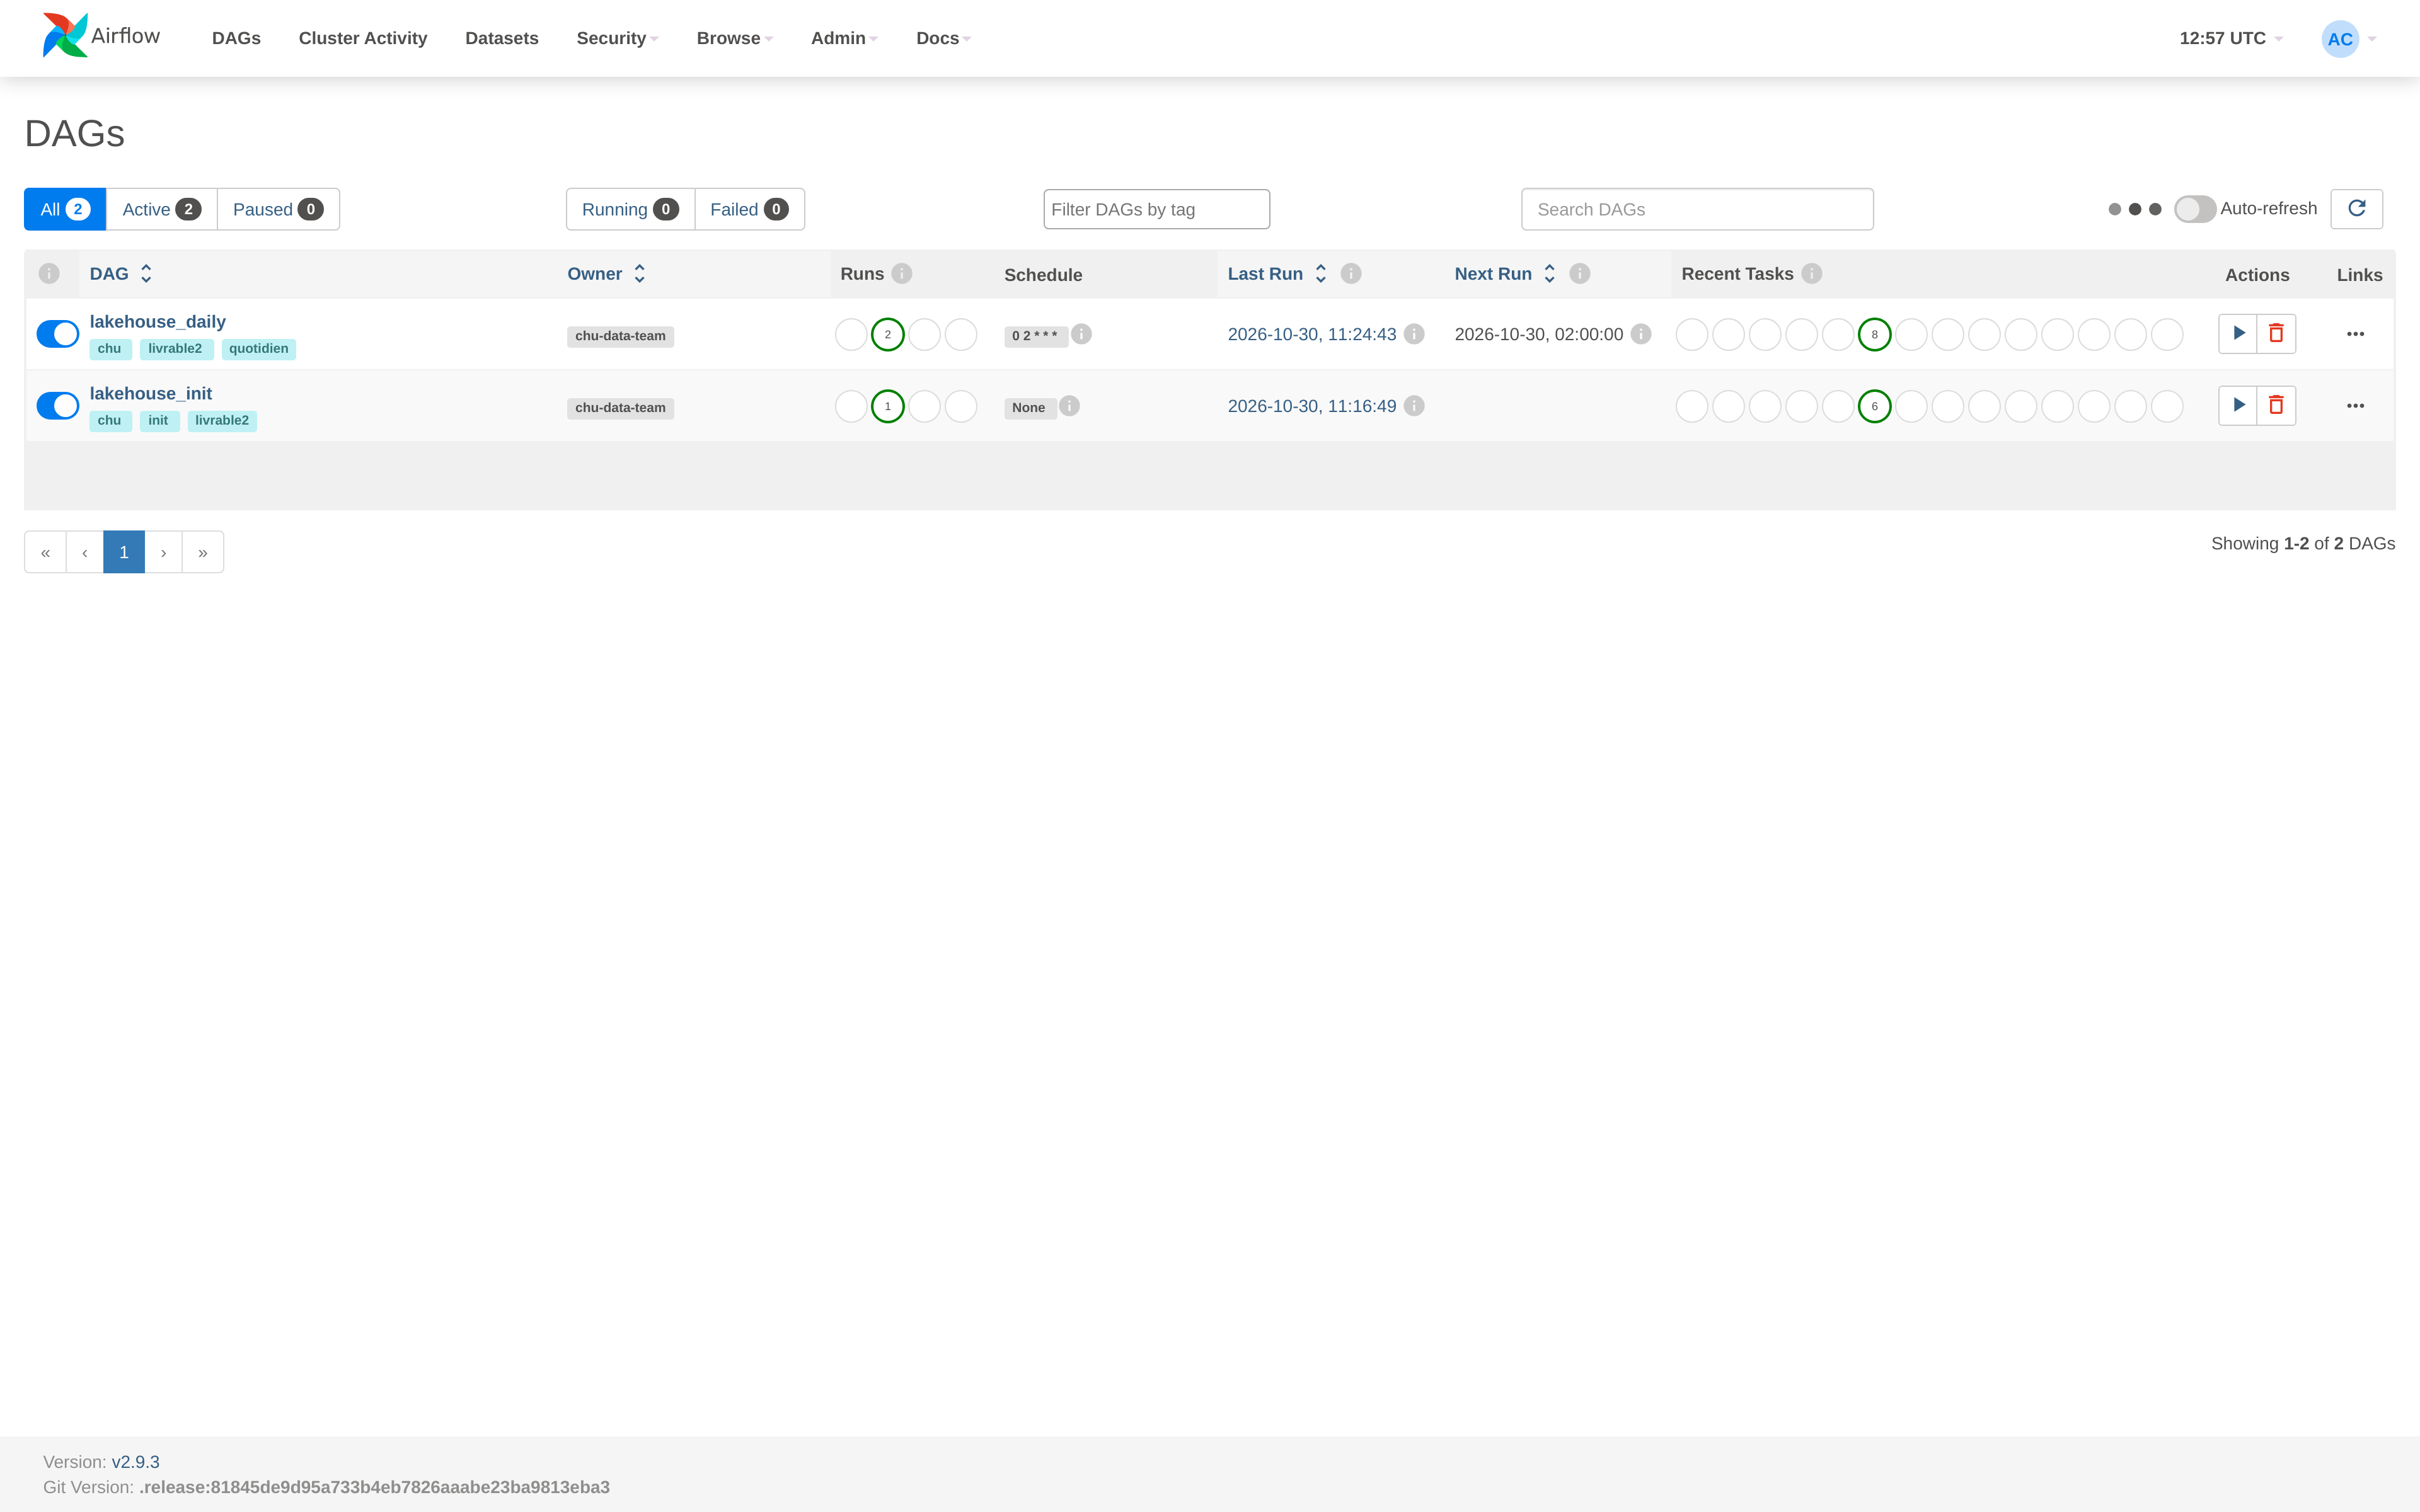
\includegraphics[width=\textwidth]{ImagesRapport/airflow_dags.png}
\end{figure}}{}

\IfFileExists{ImagesRapport/trino_query.png}{%
\begin{figure}[H]\centering
\caption{Trino 484 (UI web) : tableau de bord du coordinateur -- workers actifs et requetes recentes (etat, duree, SQL)}
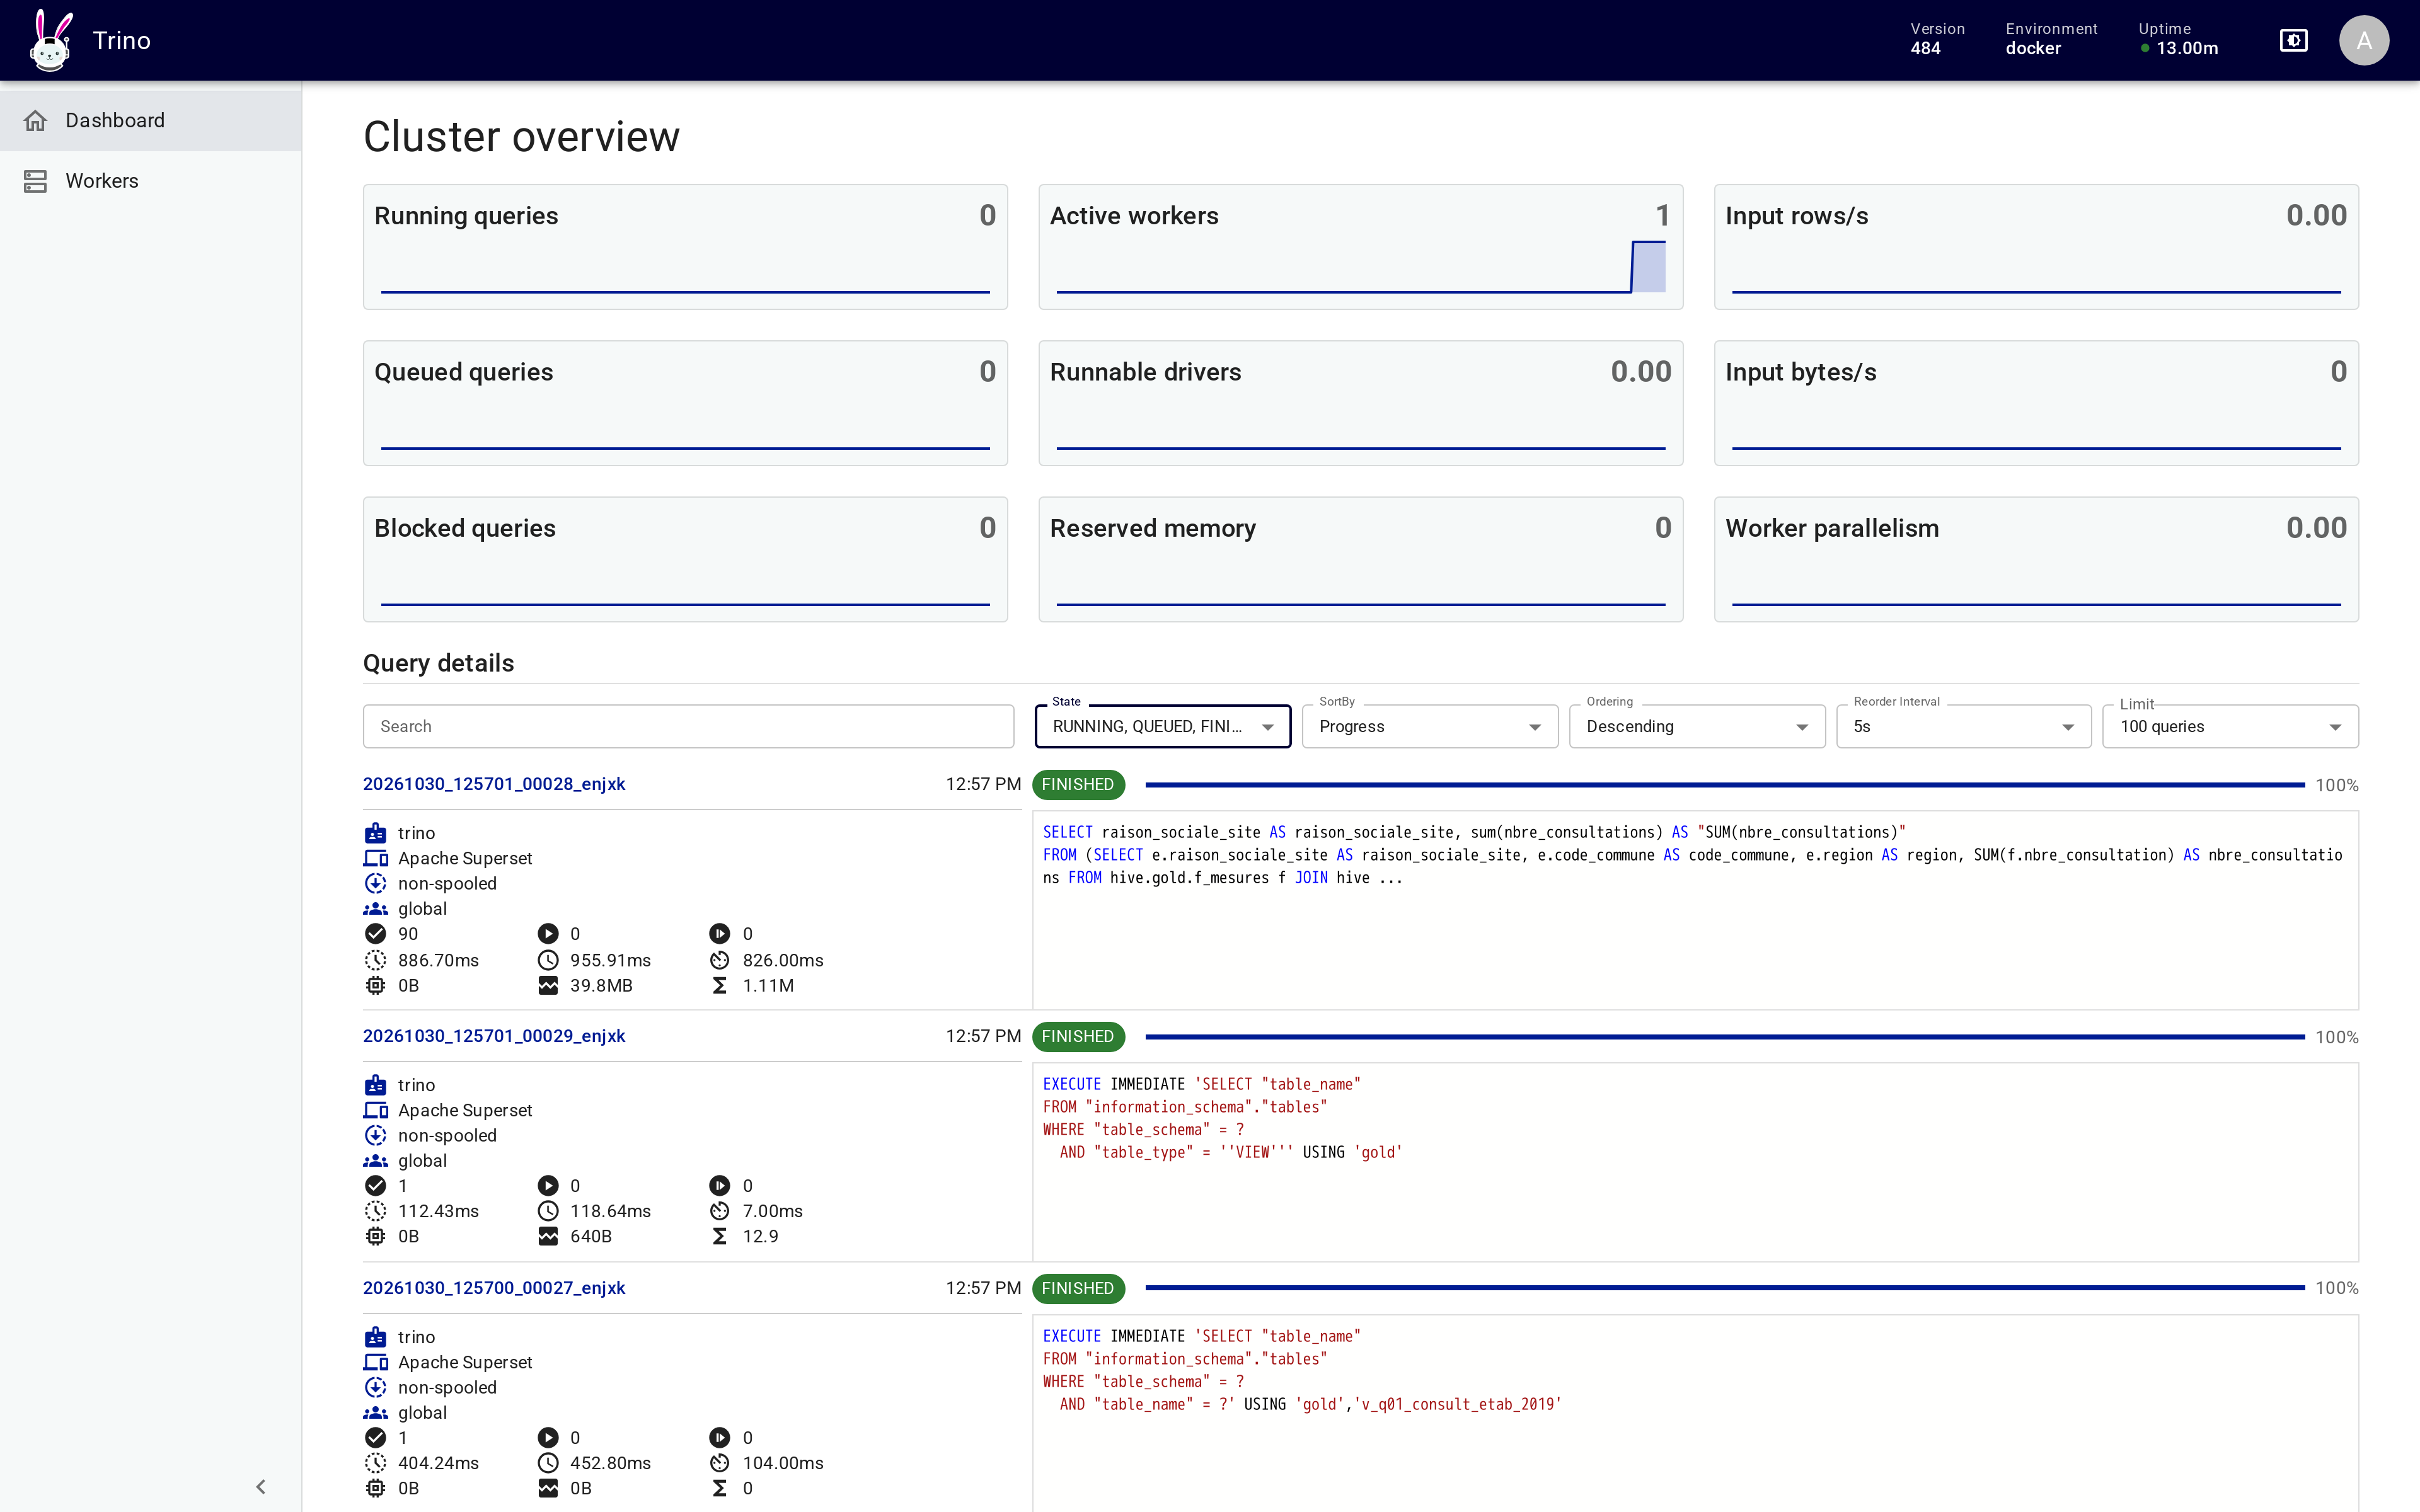
\includegraphics[width=\textwidth]{ImagesRapport/trino_query.png}
\end{figure}}{}

\IfFileExists{ImagesRapport/MInIO.png}{%
\begin{figure}[H]\centering
\caption{MinIO (console) : liste des buckets, dont \texttt{lake}}
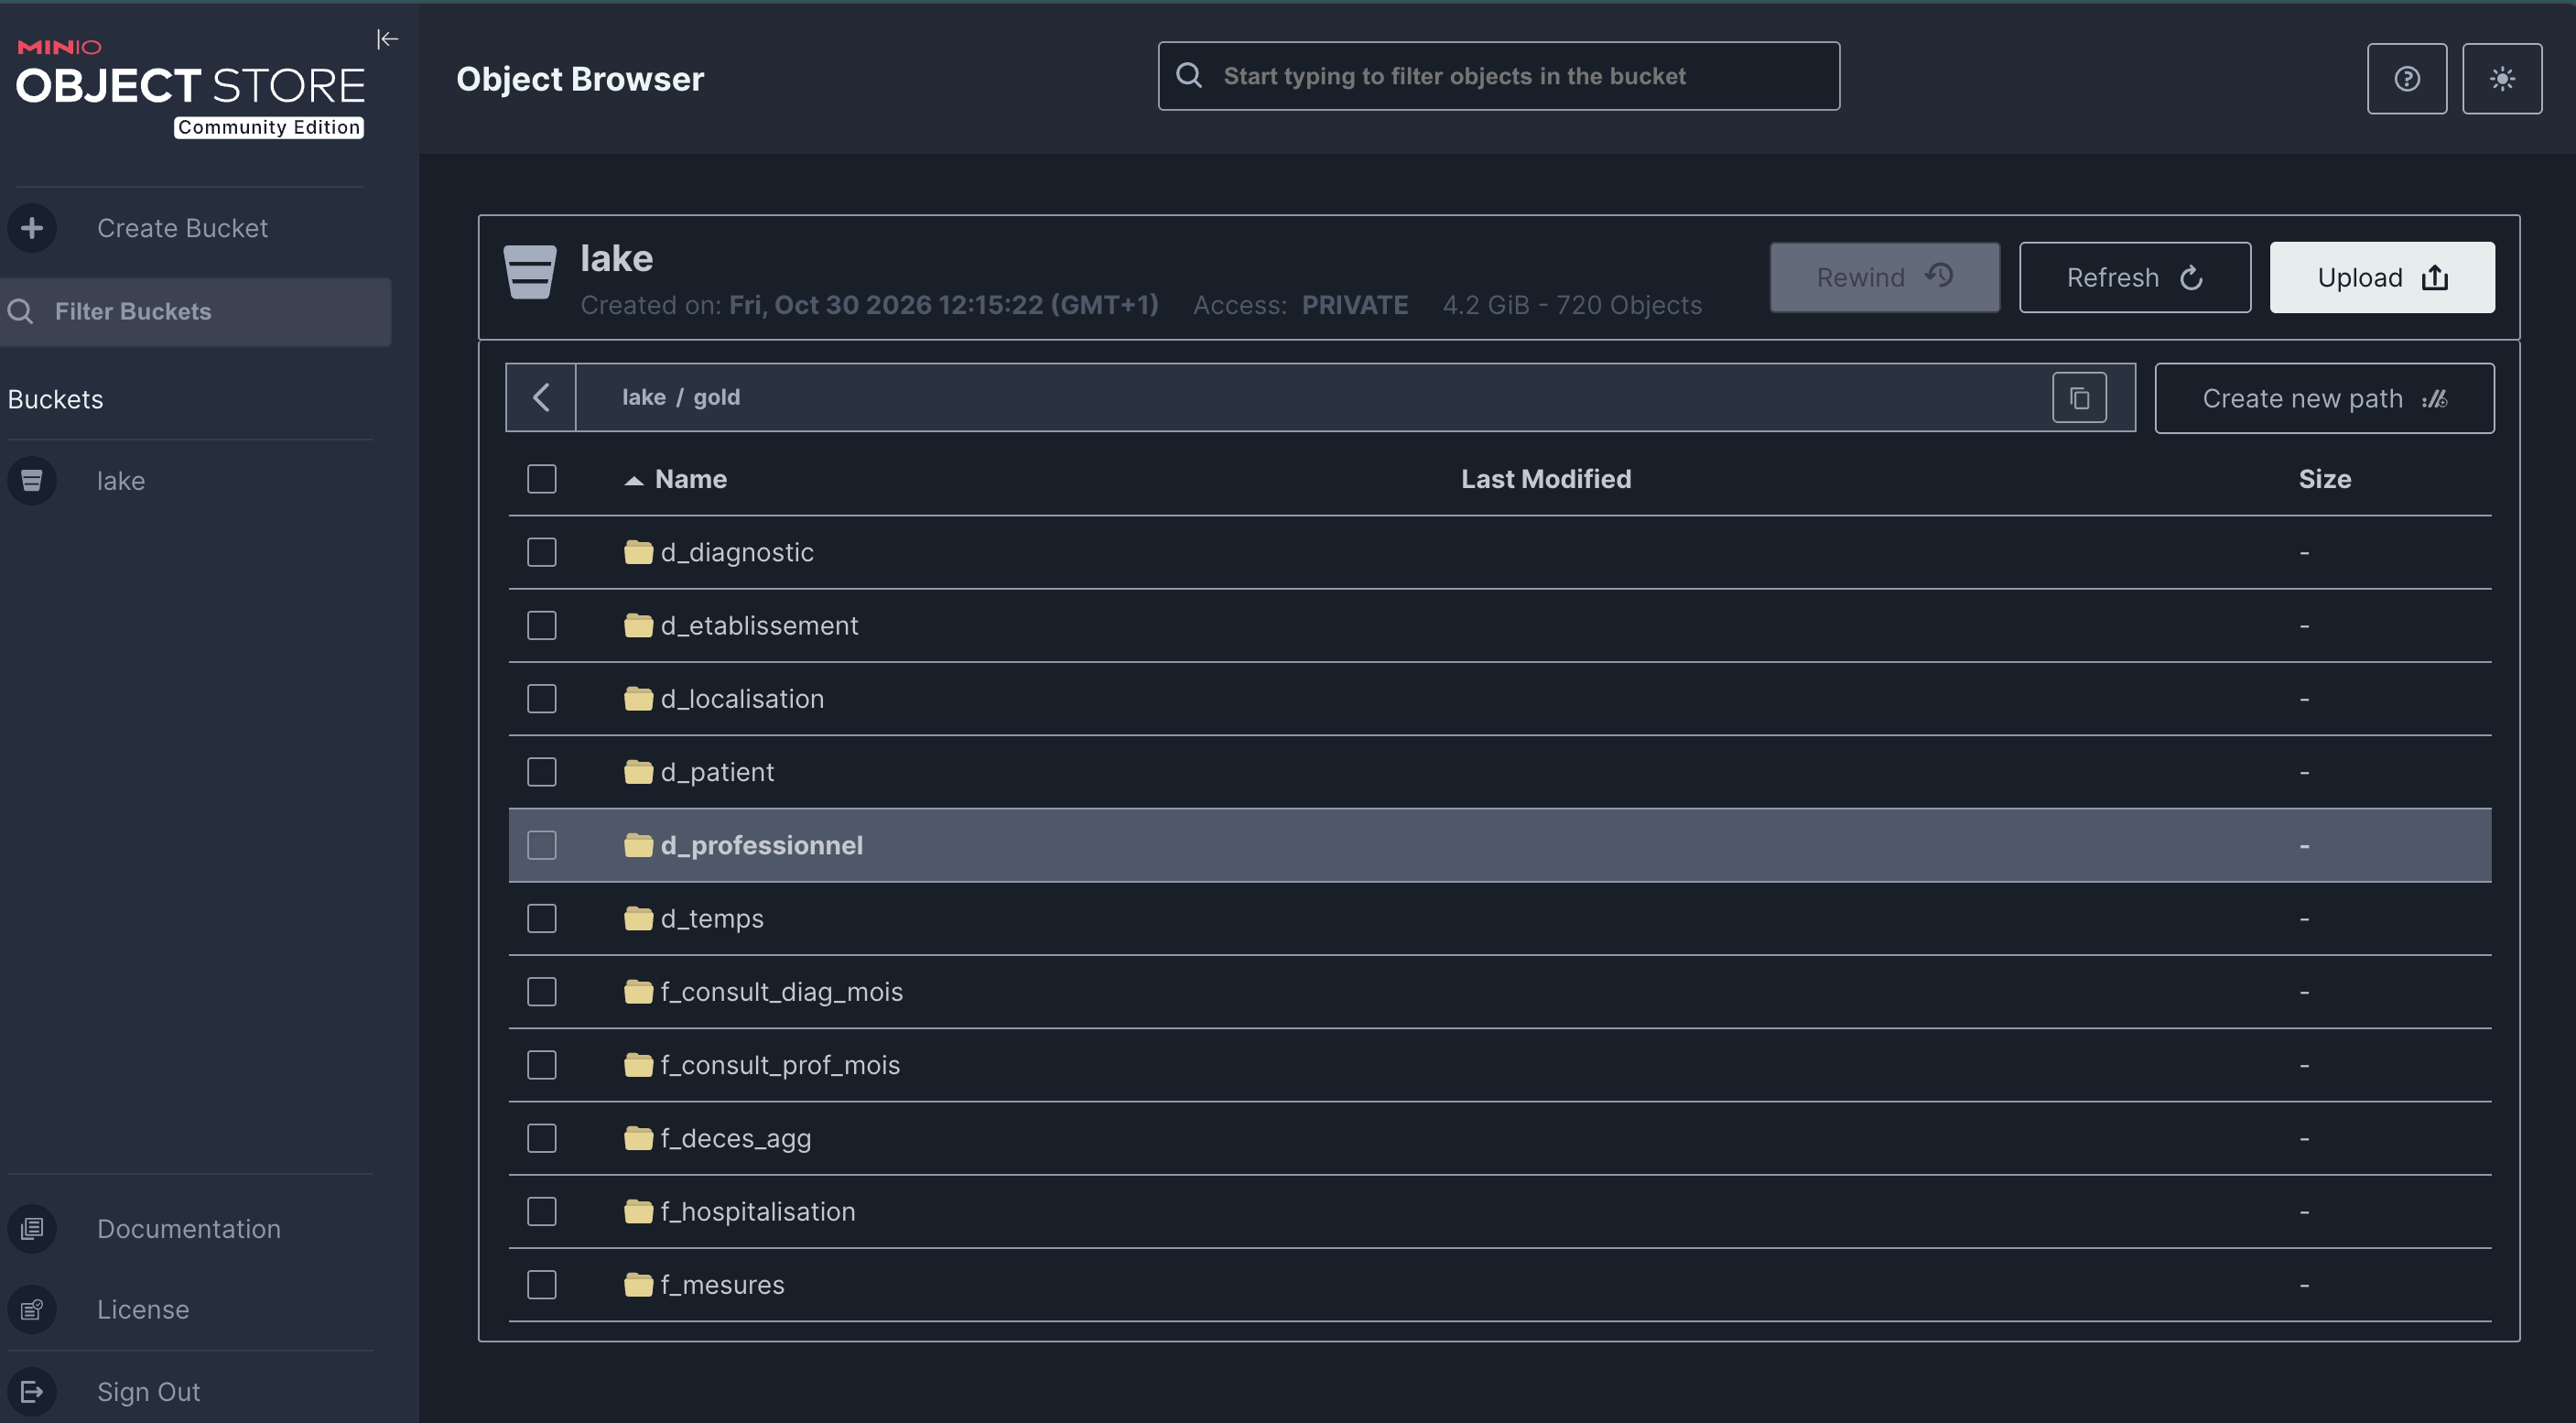
\includegraphics[width=\textwidth]{ImagesRapport/MInIO.png}
\end{figure}}{}

\IfFileExists{ImagesRapport/ManIo2.png}{%
\begin{figure}[H]\centering
\caption{MinIO (console) : contenu du bucket \texttt{lake} (zones raw/silver/gold)}
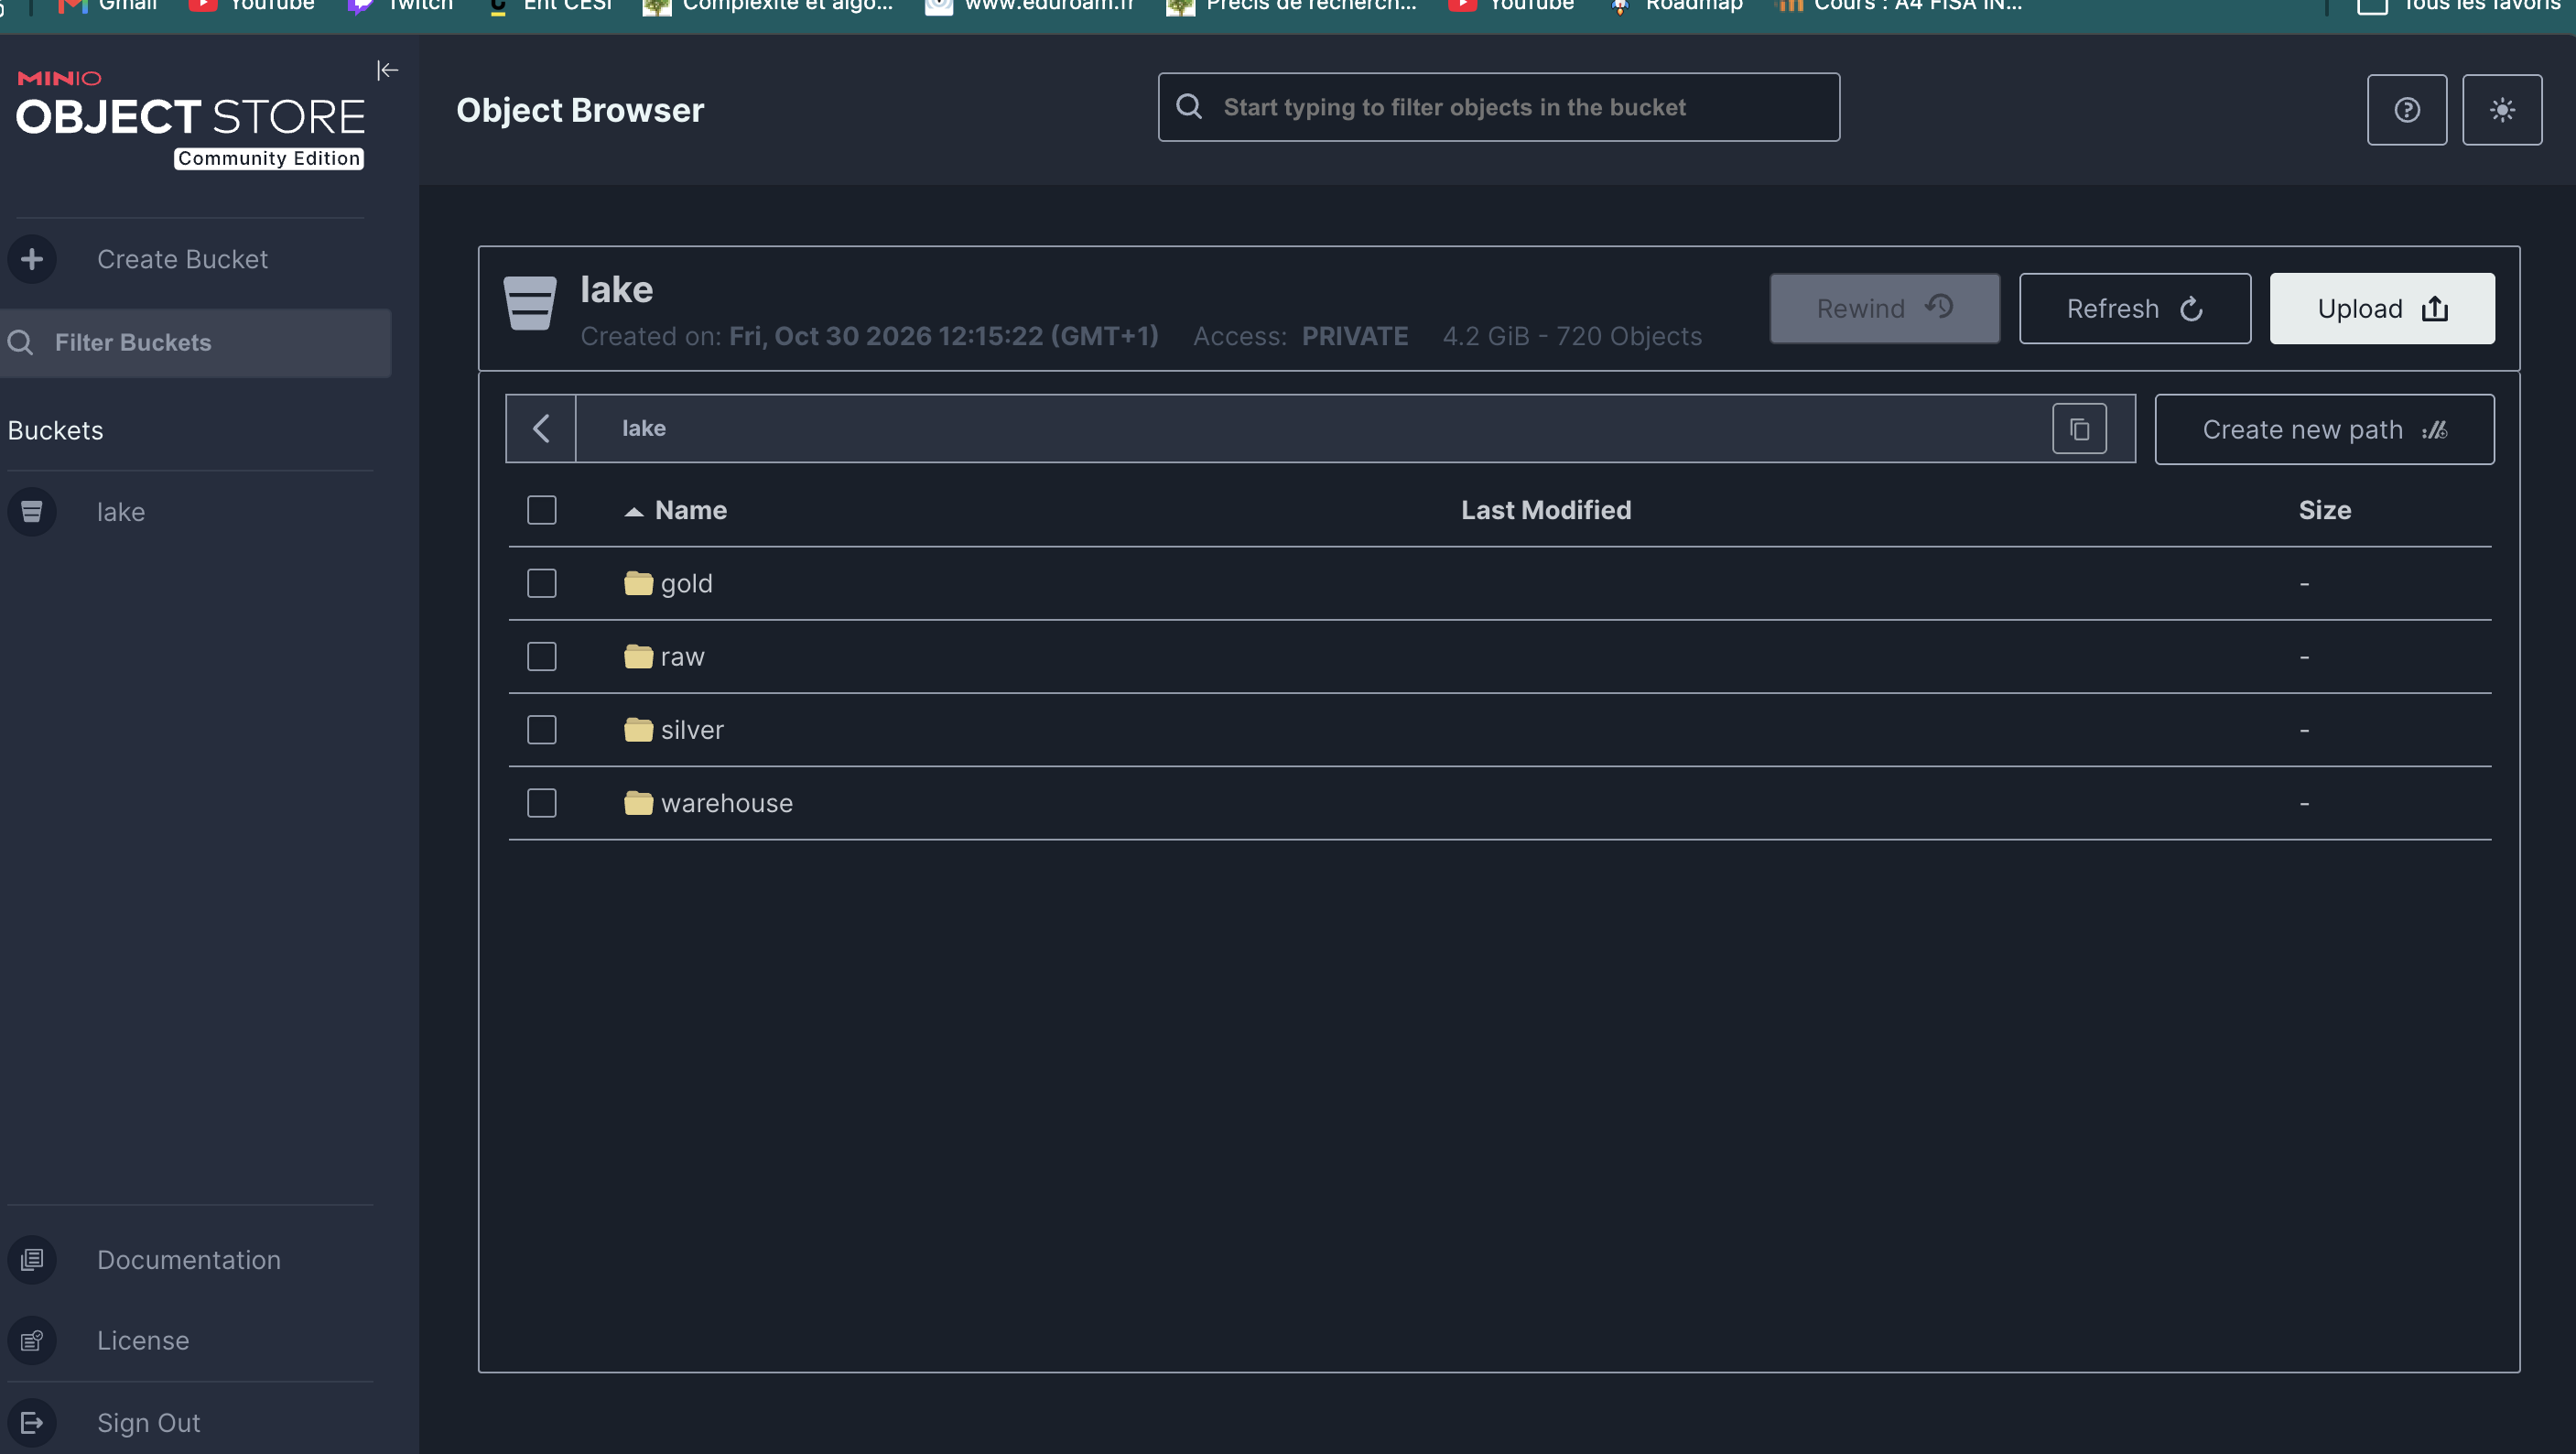
\includegraphics[width=\textwidth]{ImagesRapport/ManIo2.png}
\end{figure}}{}

\IfFileExists{ImagesRapport/probe_dash3.png}{%
\begin{figure}[H]\centering
\caption{Superset : tableau de bord \guillemotleft{}CHU -- Indicateurs metier\guillemotright{} publie (liste de ses graphiques)}
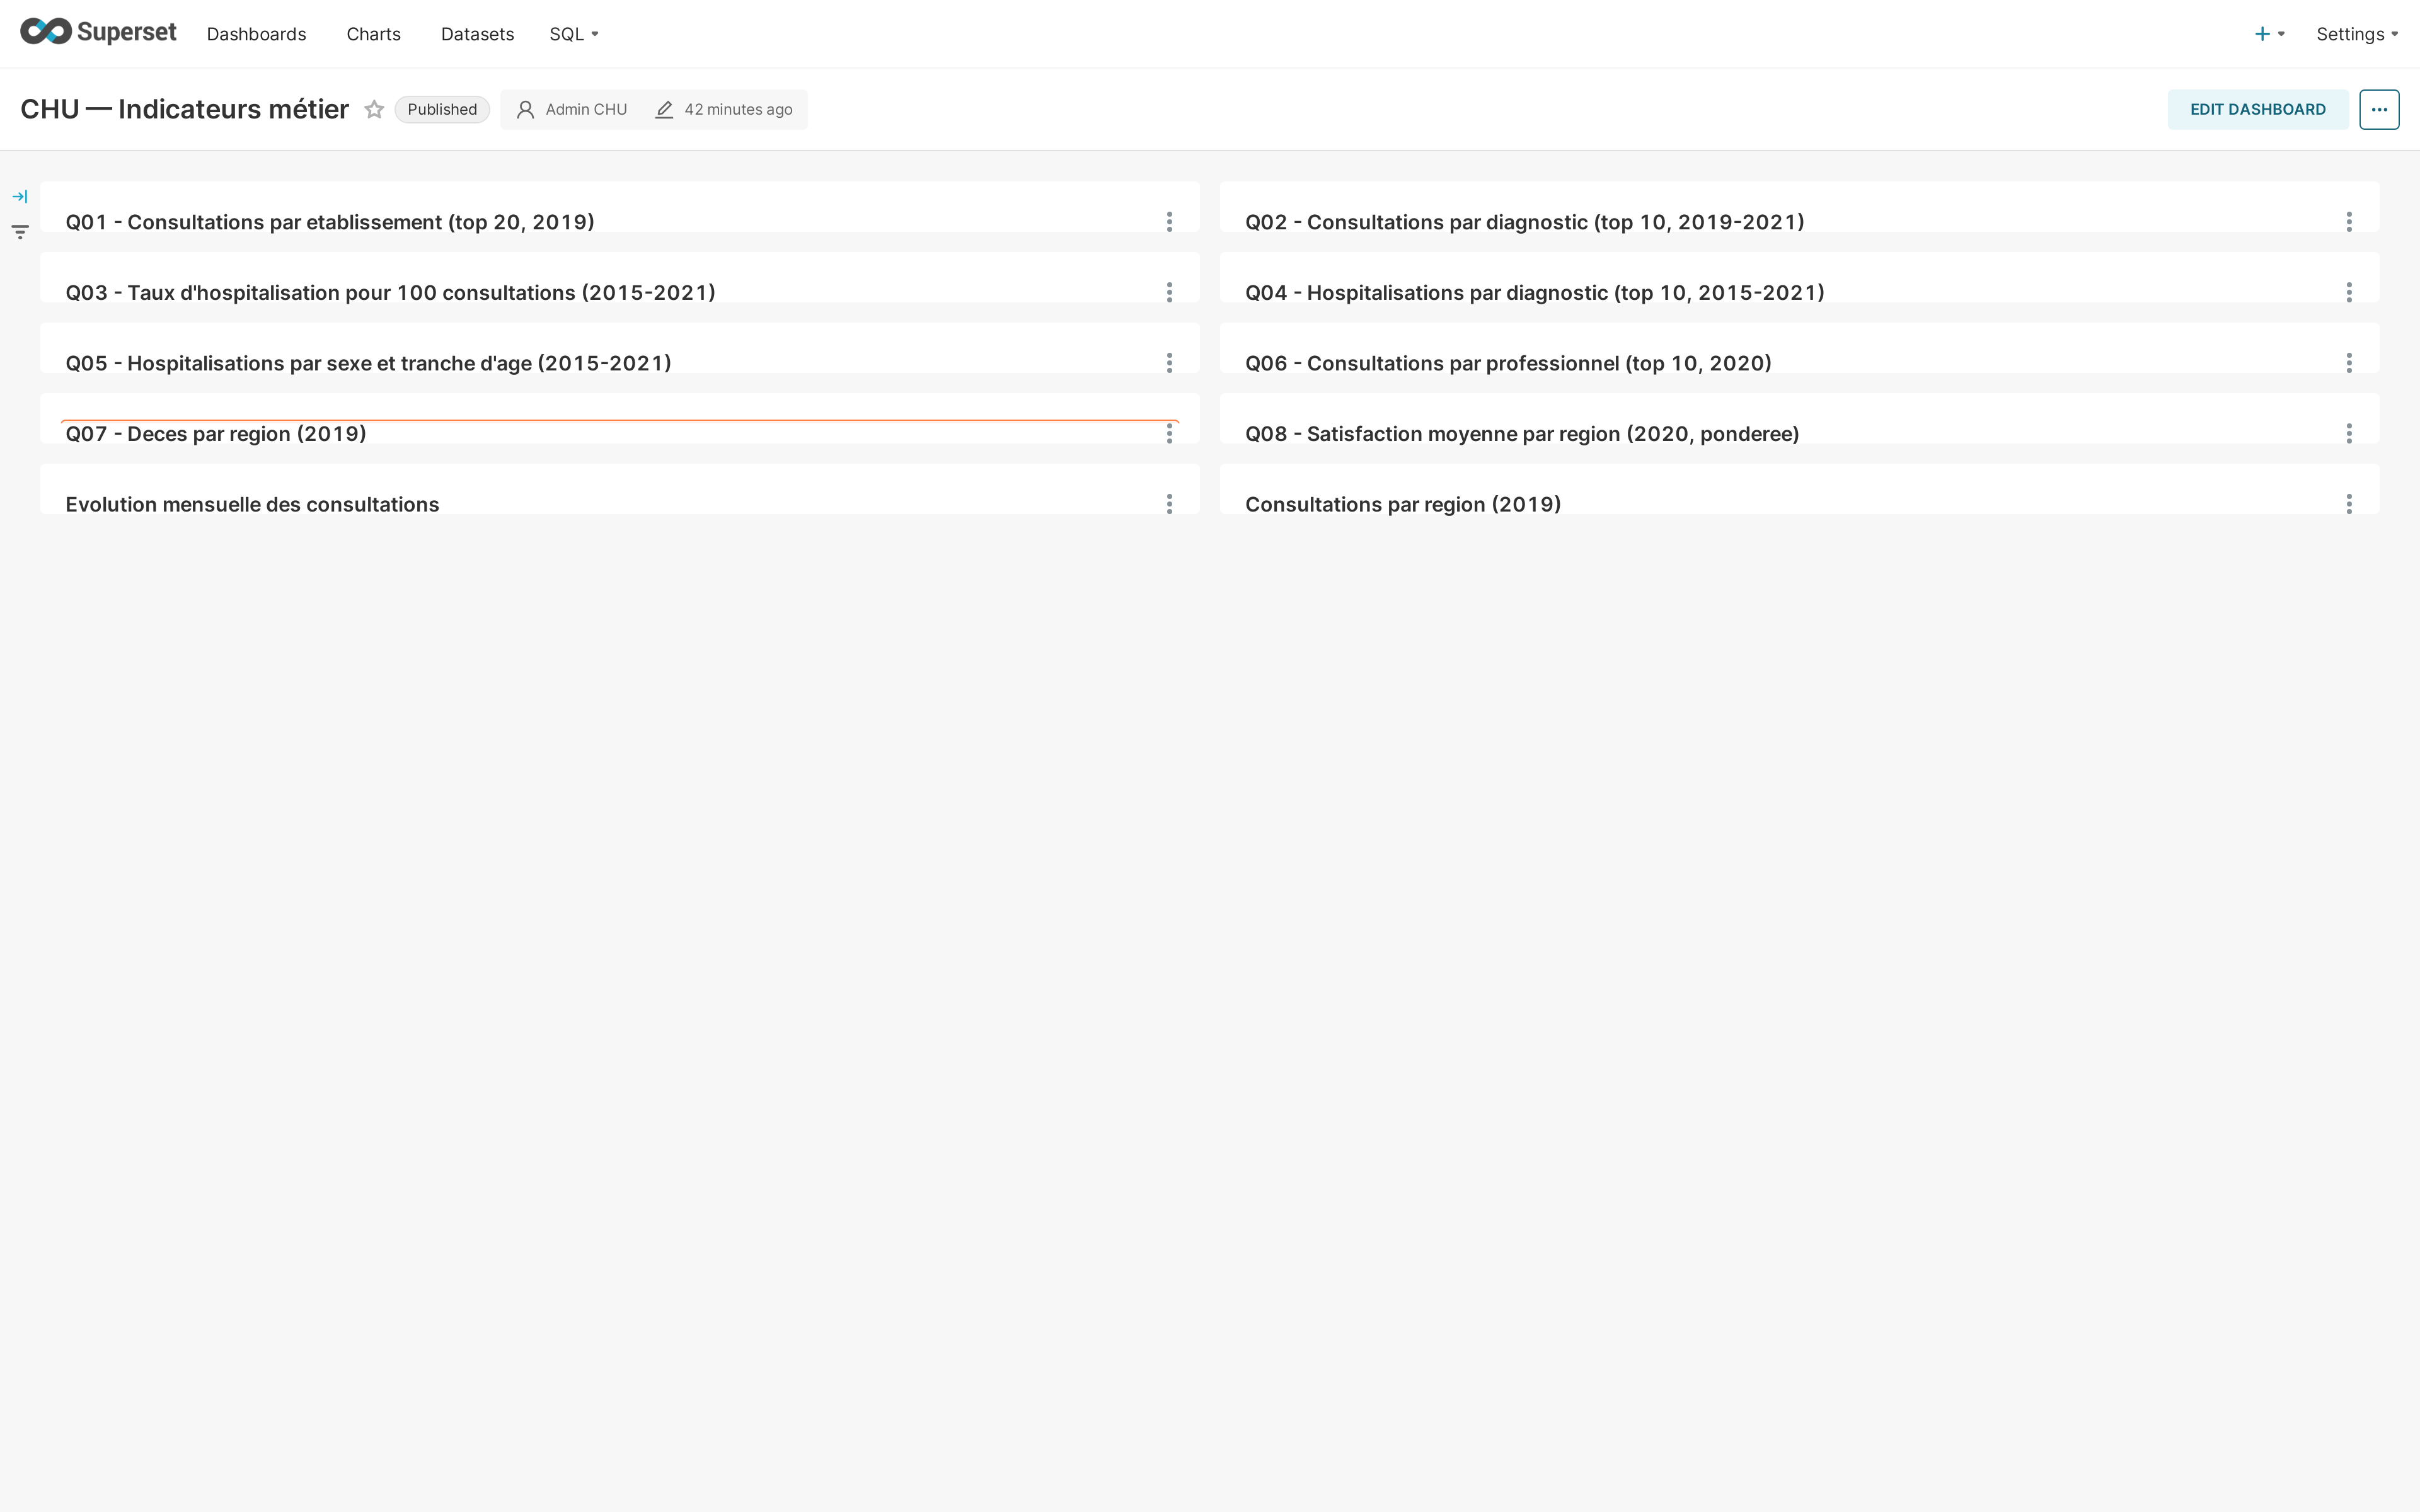
\includegraphics[width=\textwidth]{ImagesRapport/probe_dash3.png}
\end{figure}}{}

\IfFileExists{ImagesRapport/probe_dash4.png}{%
\begin{figure}[H]\centering
\caption{Superset : tableau de bord \guillemotleft{}CHU -- Indicateurs metier\guillemotright{} avec graphiques rendus}
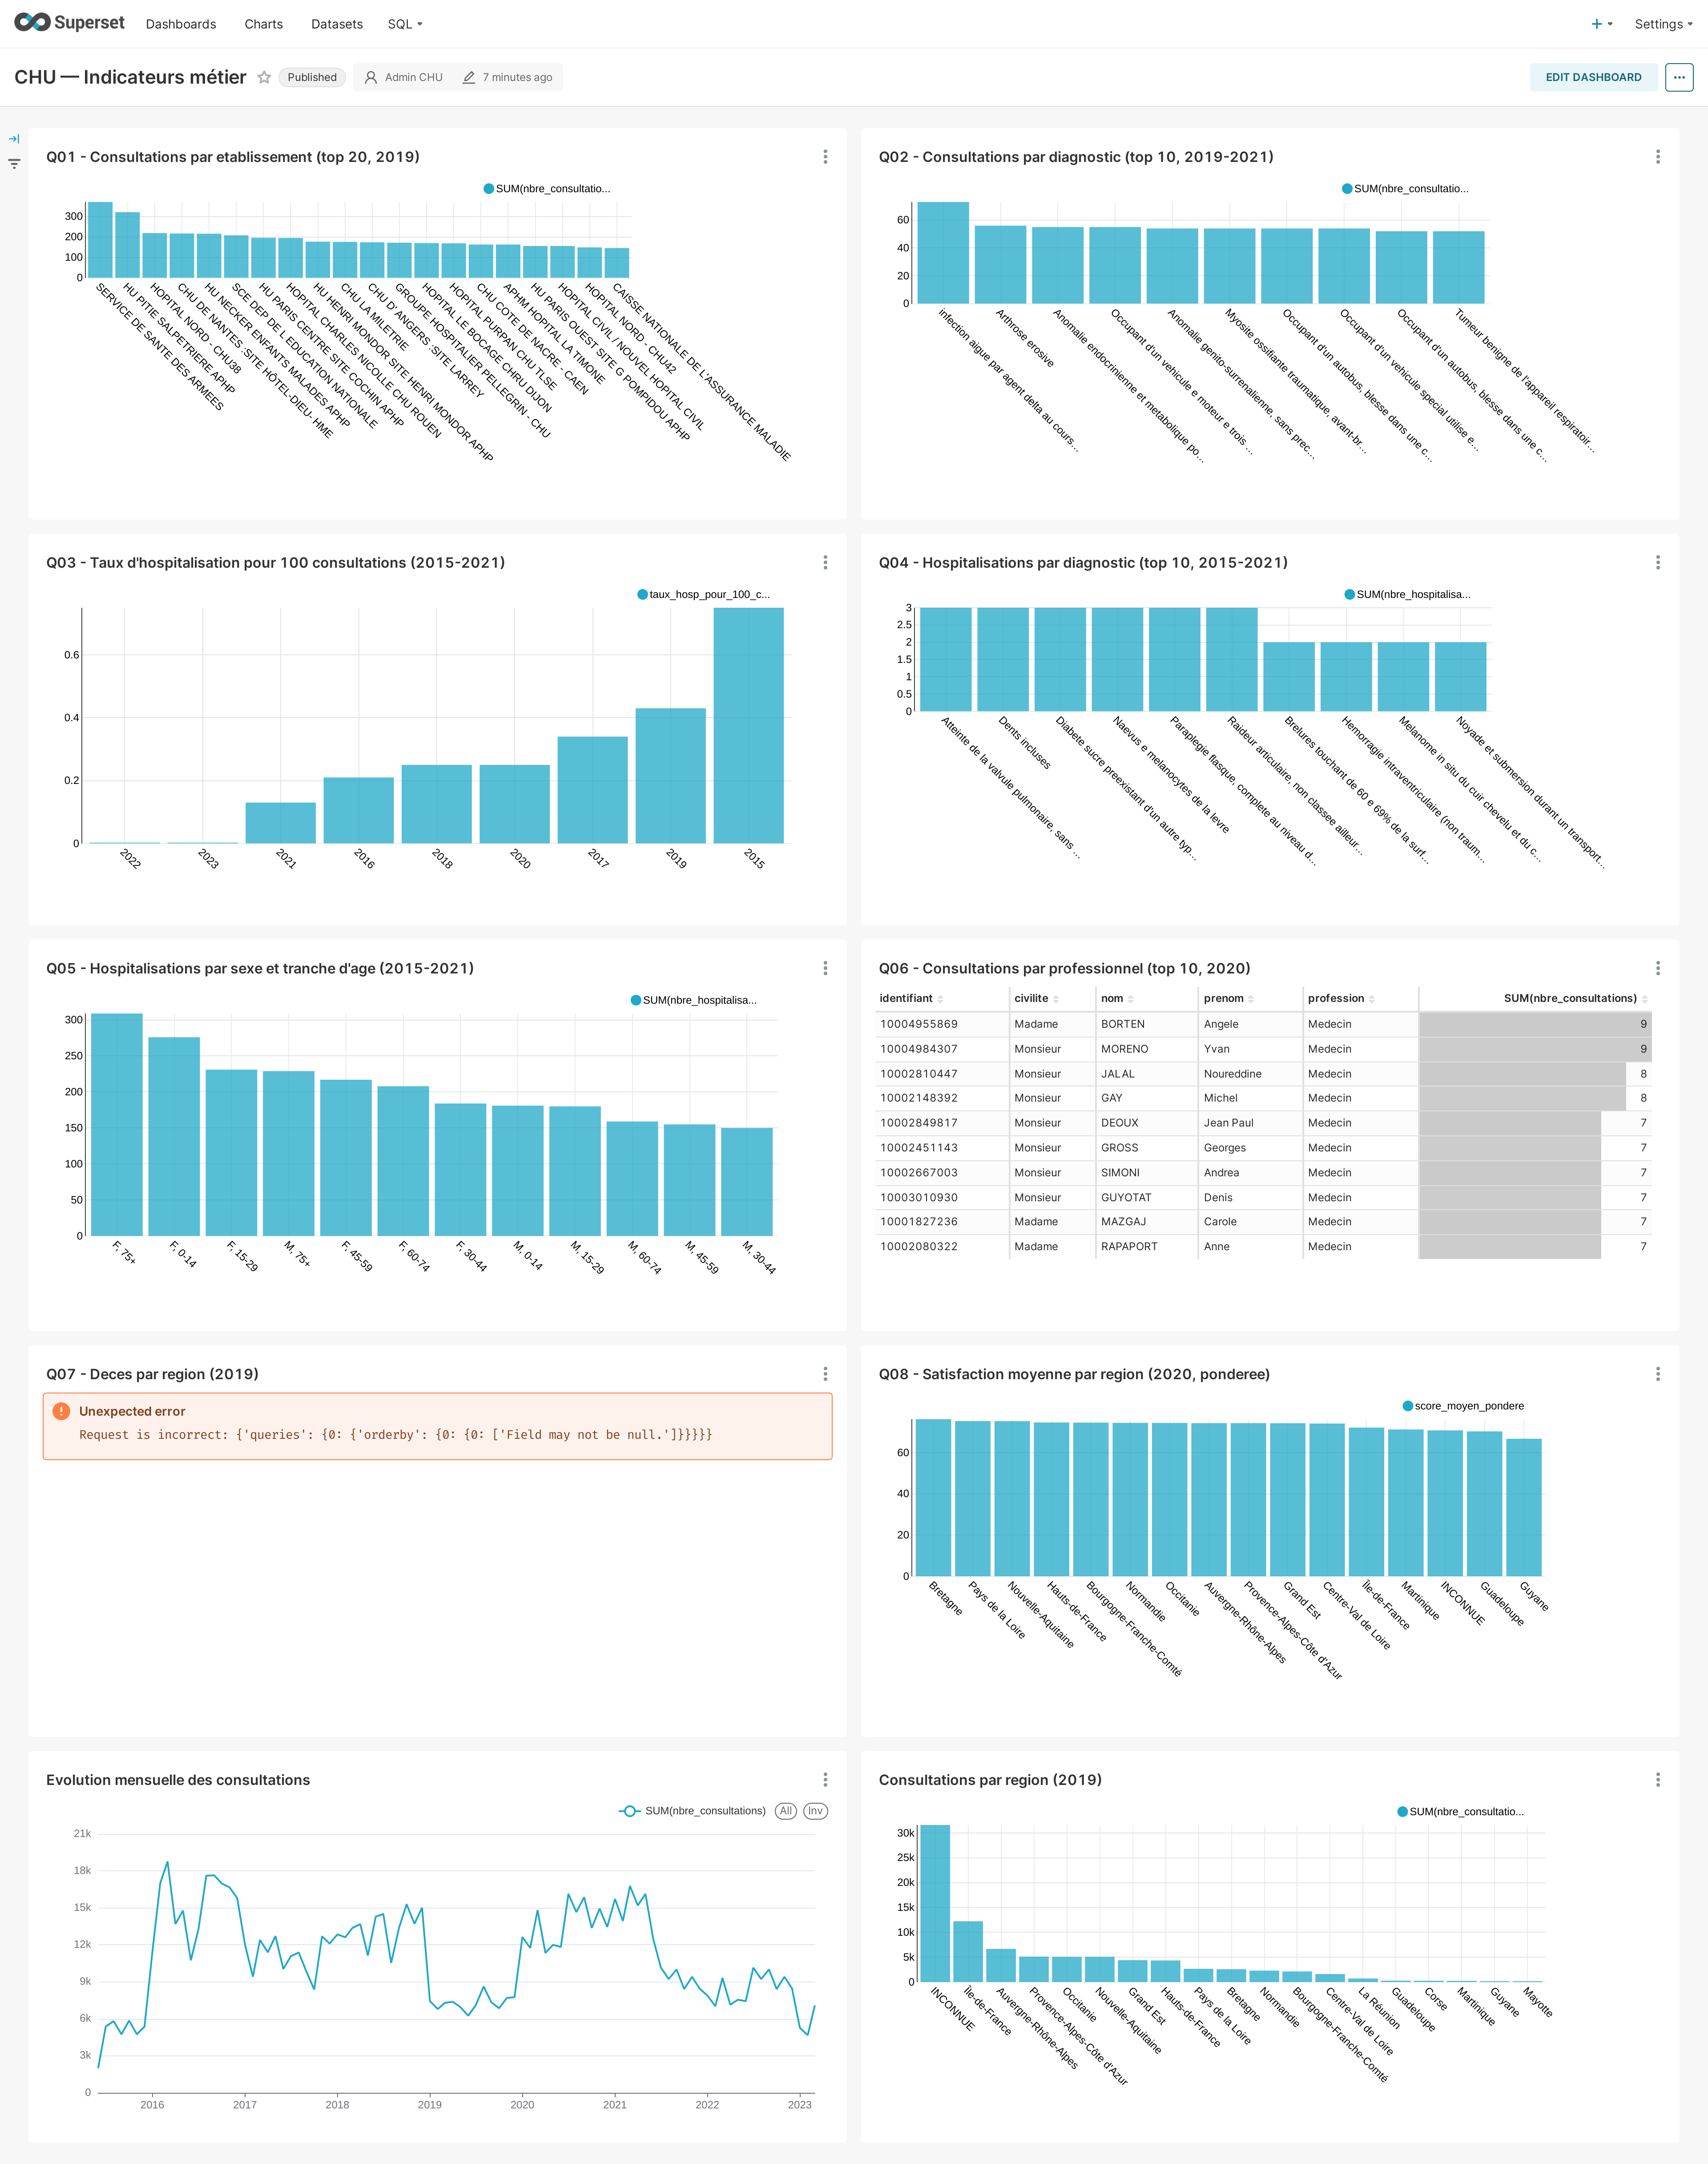
\includegraphics[width=\textwidth]{ImagesRapport/probe_dash4.png}
\end{figure}}{}

\IfFileExists{ImagesRapport/superset_chart.png}{%
\begin{figure}[H]\centering
\caption{Superset : detail d'un graphique du tableau de bord}
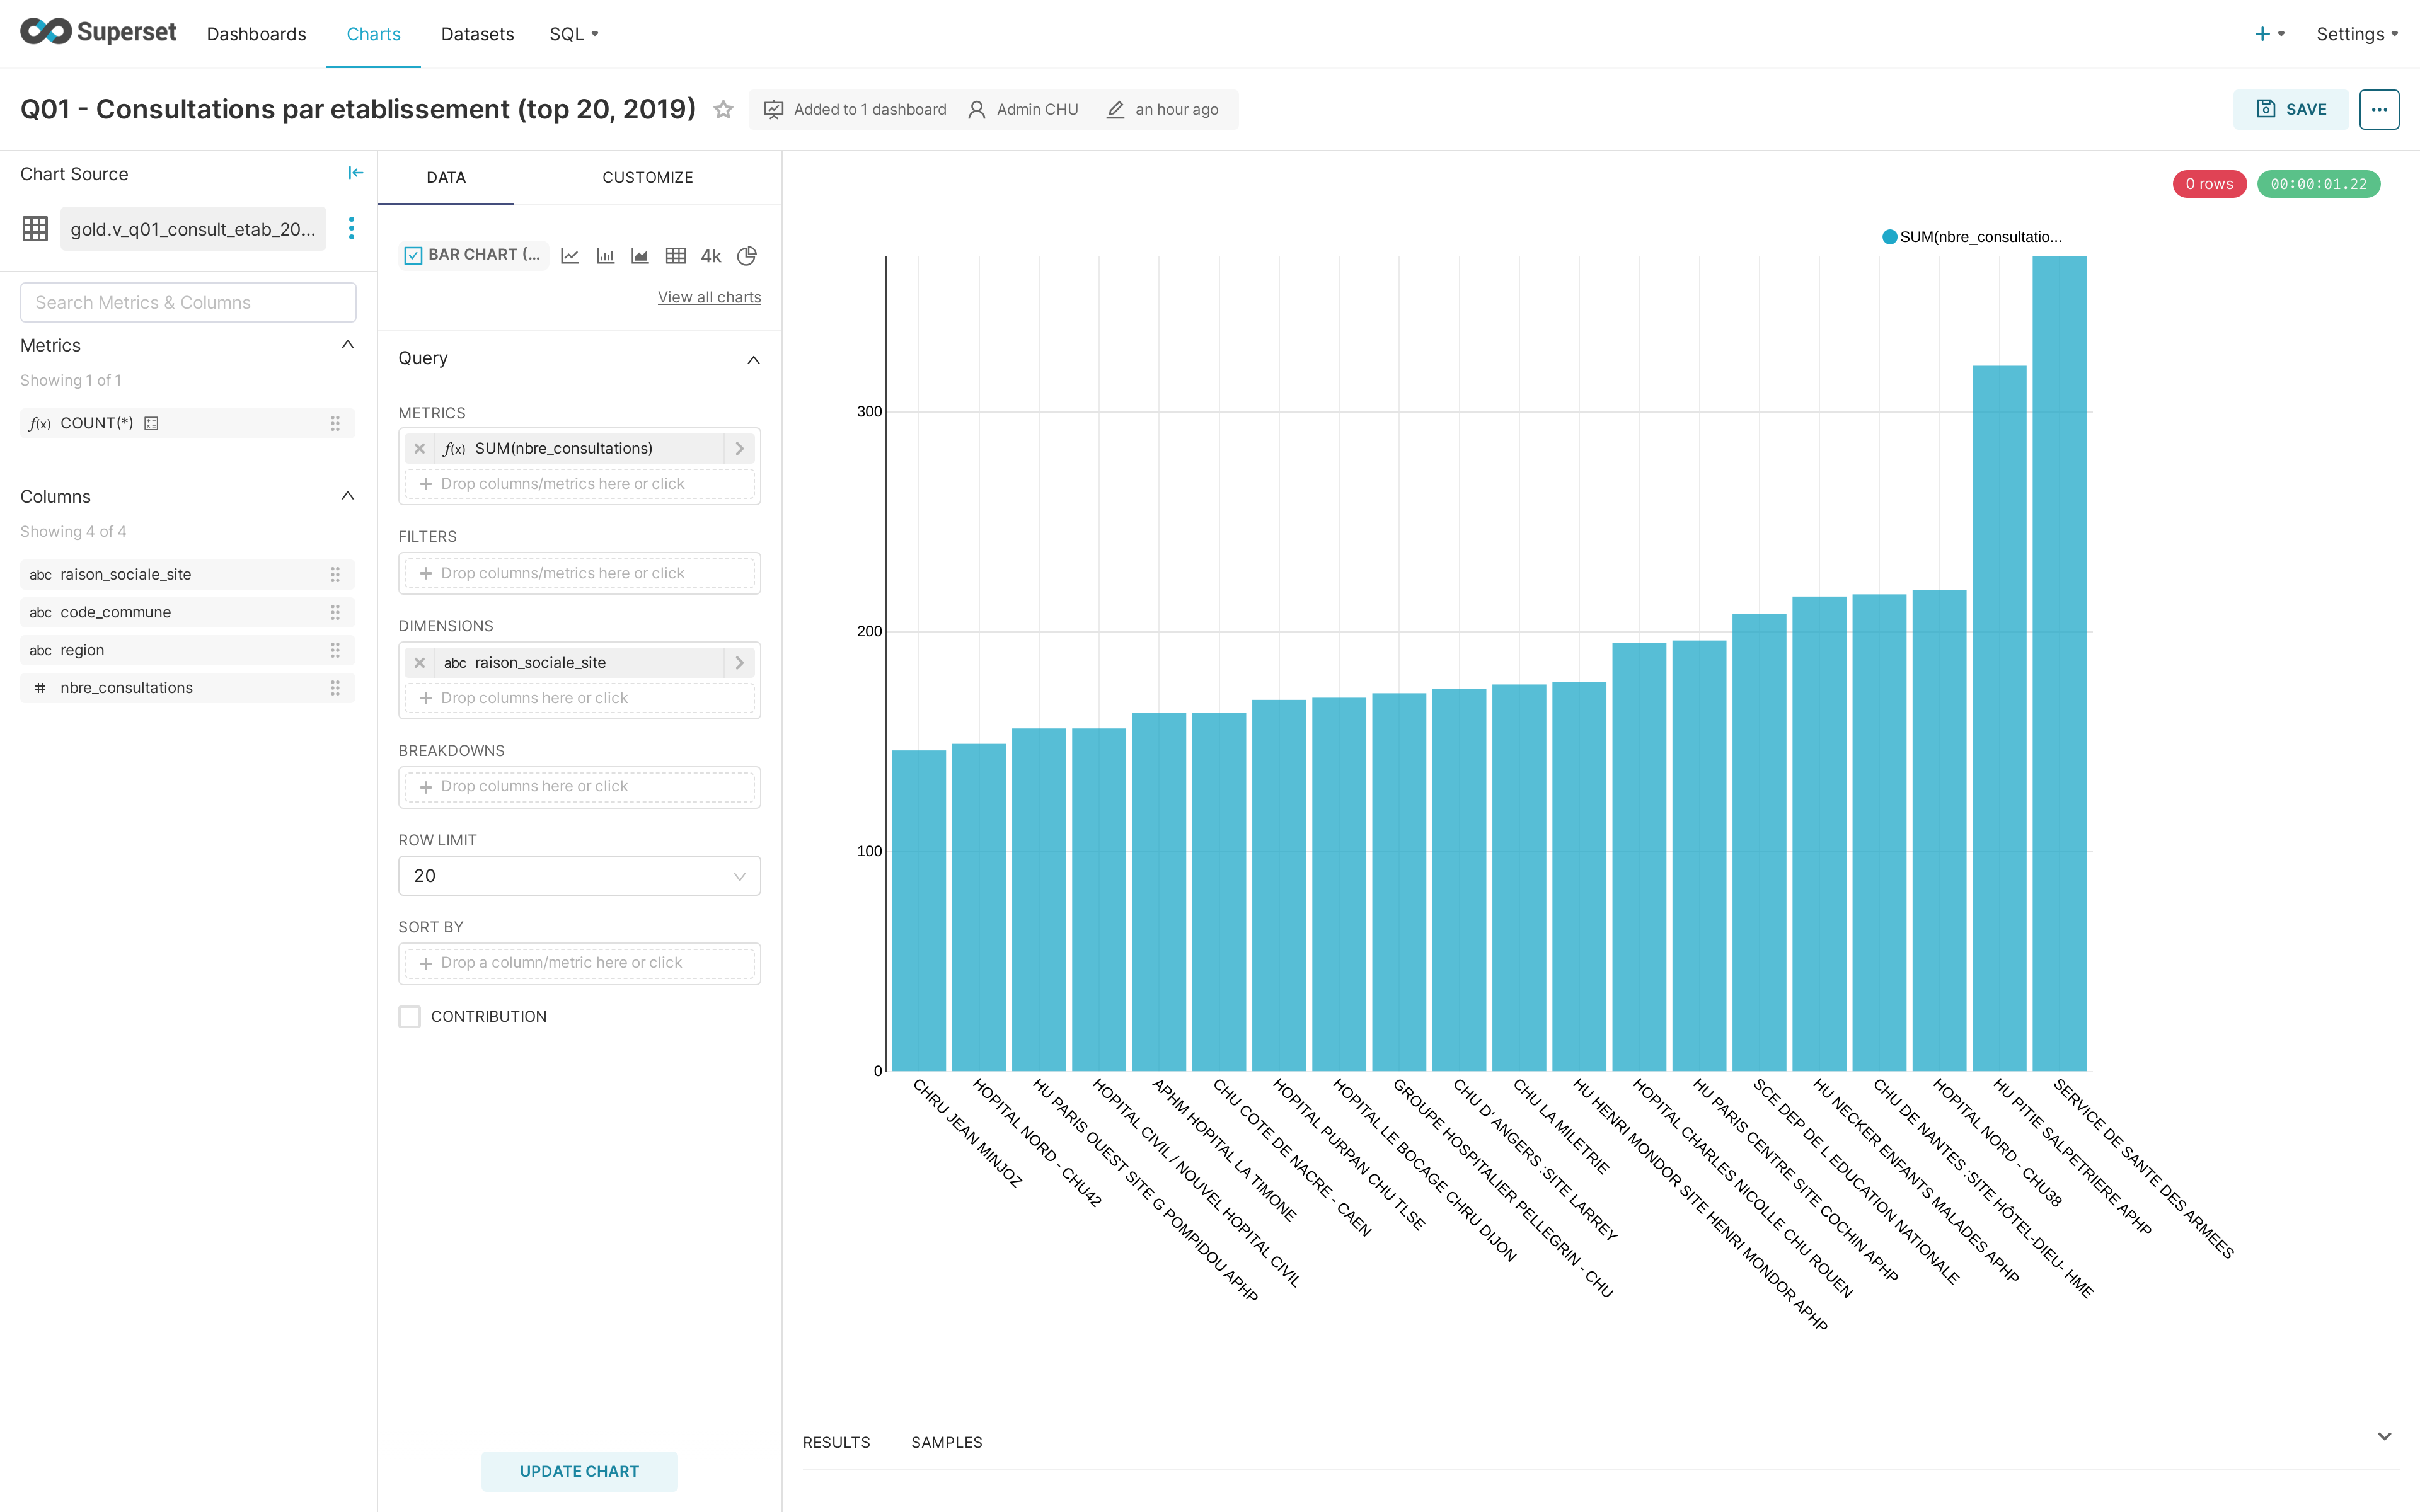
\includegraphics[width=\textwidth]{ImagesRapport/superset_chart.png}
\end{figure}}{}

% ============================ 5. PARTITIONNEMENT ============================
\section{Strategie de partitionnement et d'indexation}

\subsection{Partitionnement retenu (justifie par le moteur : Hive/Spark/Trino)}
\begin{table}[H]\centering\small
\caption{Partitionnement par table et justification}
\begin{tabular}{p{4.2cm}p{3.6cm}p{7.4cm}}
\toprule
\textbf{Table} & \textbf{Colonnes de partition} & \textbf{Justification} \\
\midrule
\texttt{f\_mesures} & \texttt{annee}, \texttt{sexe}, \texttt{tranche\_age} & pruning temporel + demographique ; les requetes metier filtrent sur l'annee/le sexe/l'age (besoins 5, 10). 9 annees $\times$ 3 sexes $\times$ 8 tranches = 216 combinaisons max (122 presentes) \\
\texttt{d\_patient} & \texttt{sexe}, \texttt{tranche\_age\_ref} & partitionnement demographique de la dimension patient \\
\texttt{d\_temps} & \texttt{annee} & partitionnement temporel 2015--2030 (couvre 2015--2021) \\
\texttt{d\_localisation} & \texttt{code\_region} & la region est l'axe geographique le plus filtrant (besoins 7, 8) ; partitionnee par \emph{code} car les noms de regions contiennent des caracteres invalides dans les chemins Hive \\
\texttt{f\_consultation\_detail}, \texttt{f\_hospitalisation}, \texttt{f\_consult\_diag\_mois}, \texttt{f\_consult\_prof\_mois} & \texttt{annee} & pruning temporel (tous les besoins portent sur des periodes) \\
\texttt{f\_deces\_agg} & \texttt{annee} seulement & sinon 1 251 combinaisons reelles (~55 lignes chacune) pour 69 008 lignes = \emph{small-files problem} ; le tri intra-partition par \texttt{(sexe, tranche\_age, id\_localisation)} compense \\
\texttt{f\_satisfaction} & \texttt{annee}, \texttt{code\_region} & grain juridique $\times$ annee ; region = colonne la plus filtrante (besoin 8), par code pour la meme raison que \texttt{d\_localisation} \\
\texttt{d\_etablissement}, \texttt{d\_diagnostic}, \texttt{d\_professionnel} & -- & peu filtrees seules ; le tri intra-fichier suffit \\
\bottomrule
\end{tabular}
\end{table}

\subsection{Pourquoi pas de bucketing (decision technique testee)}
\texttt{CLUSTERED BY (cle) INTO N BUCKETS} / \texttt{bucketBy(n, cle)} a ete
\textbf{teste puis retire} : Spark n'ecrit qu'un fichier Parquet par bucket
\emph{non vide} (avec AQE, une petite partition produit p.~ex. 2 fichiers pour
32 buckets declares) et \textbf{Trino 484 refuse alors de lire la table} a
l'execution (\guillemotleft{}number of files (N) does not match declared bucket
count (32)\guillemotright{} -- verification inconditionnelle dans le chargeur de
splits Hive). Le schema deploye est donc \textbf{partitionne + trie, sans
bucketing} : la co-localisation des lignes partageant une cle de jointure est
obtenue par le \textbf{tri intra-partition} (\texttt{sortWithinPartitions} sur
\texttt{(id\_etablissement, id\_patient)}), qui produit les statistiques min/max
par fichier Parquet alimentant le pruning intra-fichier cote Trino.

\subsection{Indexation complementaire}
\begin{itemize}[leftmargin=*]
\item \textbf{Parquet + Zstd} : format colonnaire compresse ($\times$5 a $\times$10 vs CSV),
      pushdown des predicats, statistiques min/max par colonne et par fichier $\rightarrow$
      pruning intra-fichier (Trino) en plus du pruning de partitions ;
\item \textbf{tri intra-partition} sur les cles de jointure (\texttt{sortWithinPartitions}) ;
\item \textbf{statistiques} : \texttt{ANALYZE TABLE ... COMPUTE STATISTICS} (Hive/Spark) et
      \texttt{ANALYZE} (Trino) apres chaque chargement $\rightarrow$ plans de jointure optimaux ;
\item \textbf{agregats pre-calcules} (\texttt{f\_consult\_diag\_mois}, \texttt{f\_consult\_prof\_mois}) :
      equivalents materialises des aggregations les plus demandees (besoins 2 et 6) ;
\item \textbf{aggregation en amont} du fait deces (25,09 M $\rightarrow$ 69 008 lignes) : le grain
      annuel evite de scanner 25 M de lignes pour un besoin annuel.
\end{itemize}

% ============================ 6. QUALITE ====================================
\section{Rapport de qualite des donnees integrees}

8 familles de controles qualite produisent 9 rapports. Les controles sur les
sources definissent les regles de traitement (\S5.7) ; les controles
\guillemotleft{}doublons faits\guillemotright{}, \guillemotleft{}completude par
attribut\guillemotright{} et \guillemotleft{}integrite FK\guillemotright{} portent
sur les \textbf{donnees integrees} (Parquet Gold/Silver du lake lus en direct),
comme l'exige le sujet.

\subsection{Completude par attribut -- sources}
{\small\begin{longtable}{p{3.0cm}p{5.0cm}rrr}
\caption{Completude par attribut -- sources}\\
\toprule
\textbf{Fichier} & \textbf{Attribut} & \textbf{Total} & \textbf{Non vide} & \textbf{\%} \\
\midrule
\endfirsthead
\toprule
\textbf{Fichier} & \textbf{Attribut} & \textbf{Total} & \textbf{Non vide} & \textbf{\%} \\
\midrule
\endhead
\rowsdqcompletude
\bottomrule
\end{longtable}}

\subsection{Completude par attribut -- faits integres (lake)}
{\small\setlength{\tabcolsep}{4pt}\begin{longtable}{p{4.6cm}p{4.0cm}rrr}
\caption{Completude par attribut -- faits integres Gold/Silver}\\
\toprule
\textbf{Table} & \textbf{Attribut} & \textbf{Total} & \textbf{Non null} & \textbf{\%} \\
\midrule
\endfirsthead
\toprule
\textbf{Table} & \textbf{Attribut} & \textbf{Total} & \textbf{Non null} & \textbf{\%} \\
\midrule
\endhead
\rowsdqcompletudefaits
\bottomrule
\end{longtable}}

\subsection{Validite des formats}
\begin{longtable}{p{3cm}p{5.2cm}rrr}
\caption{Validite des formats}\\
\toprule
\textbf{Fichier} & \textbf{Controle} & \textbf{Total} & \textbf{Invalides} & \textbf{\%} \\
\midrule
\endfirsthead
\toprule
\textbf{Fichier} & \textbf{Controle} & \textbf{Total} & \textbf{Invalides} & \textbf{\%} \\
\midrule
\endhead
\rowsdqvalidite
\bottomrule
\end{longtable}

\subsection{Doublons -- sources puis faits integres}
\begin{table}[H]\centering\small
\caption{Doublons sur les sources}
\begin{tabular}{p{3.4cm}p{5.8cm}rrr}
\toprule
\textbf{Fichier} & \textbf{Cle} & \textbf{Total} & \textbf{Doublons} & \textbf{\%} \\
\midrule
\rowsdqdoublons
\bottomrule
\end{tabular}
\end{table}

\begin{table}[H]\centering\small
\caption{Doublons sur les faits integres du lake}
\begin{tabular}{p{4.2cm}p{4.4cm}rrr}
\toprule
\textbf{Fait integre} & \textbf{Cle (grain)} & \textbf{Total} & \textbf{Doublons} & \textbf{\%} \\
\midrule
\rowsdqdoublonsfaits
\bottomrule
\end{tabular}
\end{table}

Deux defauts de grain detectes par ces controles ont ete corriges et le chargement
re-joue : (1) \textbf{fan-out de la jointure \texttt{activite}} (1-N) dupliquant les
consultations (1 373 594 lignes pour 1 027 157 consultations, +33,7 \,\%) $\rightarrow$
jointure ramenee a 1 organisation par professionnel (\texttt{MIN(identifiant\_organisation)}) ;
(2) \textbf{grain \texttt{f\_satisfaction}/\texttt{f\_mesures}} : le fichier ESATIS contient
plusieurs lignes (sites) par finess juridique (2 295 lignes pour 1 960 finess juridiques)
$\rightarrow$ agregation au grain juridique, moyenne ponderee par les repondants
(\texttt{SUM(score $\times$ nb\_rep) / SUM(nb\_rep)}) ; la satisfaction etant rattachee a la
region, l'absence de \texttt{region} dans la cle de \texttt{f\_mesures} produisait 31
doublons $\rightarrow$ \texttt{region} ajoutee au grain (cle a 7 colonnes, 0 doublon).
Note : la cle deces est construite avec \texttt{COALESCE(champ,'')} -- sans
\texttt{COALESCE}, un champ NULL exclut la ligne du \texttt{COUNT(DISTINCT)} et gonfle
artificiellement le compte (artefact avant correction : 211 833 = 0,8444 \,\% ;
valeur retenue : 174 794 = 0,6967 \,\%).

\subsection{Coherence referentielle -- codes FINESS}
\begin{longtable}{p{8.2cm}rrr}
\caption{Coherence referentielle FINESS sur les sources}\\
\toprule
\textbf{Controle} & \textbf{Total} & \textbf{Trouves} & \textbf{\%} \\
\midrule
\endfirsthead
\toprule
\textbf{Controle} & \textbf{Total} & \textbf{Trouves} & \textbf{\%} \\
\midrule
\endhead
\rowsdqreferentiel
\bottomrule
\end{longtable}

Points marquants : \texttt{Hospitalisations.identifiant\_organisation} $\rightarrow$
referentiel etablissement : \textbf{100,0 \,\%} ; rattachement chaine complete
consultation $\rightarrow$ professionnel $\rightarrow$ activite $\rightarrow$ etablissement :
\textbf{63,87 \,\%} (71,87 \,\% jusqu'au fichier d'activite) ; \texttt{finess\_site} quasi
vide (0,05 \,\%) et ESATIS = finess \emph{juridique} (49,91/50,74 \,\% de match,
0 \,\% en \texttt{identifiant\_organisation}) $\rightarrow$ satisfaction stockee au grain
juridique rattachee a la region.

\begin{longtable}{p{8.2cm}rrr}
\caption{Integrite referentielle faits integres $\rightarrow$ dimensions}\\
\toprule
\textbf{Controle} & \textbf{Total} & \textbf{Trouves} & \textbf{\%} \\
\midrule
\endfirsthead
\toprule
\textbf{Controle} & \textbf{Total} & \textbf{Trouves} & \textbf{\%} \\
\midrule
\endhead
\rowsdqintegritefk
\bottomrule
\end{longtable}

\subsection{Temporalité}
{\small\setlength{\tabcolsep}{2.5pt}\begin{longtable}{p{3.2cm}p{3.8cm}rrrp{3.4cm}}
\caption{Coherence temporelle}\\
\toprule
\textbf{Fichier} & \textbf{Controle} & \textbf{Total} & \textbf{Conformes} & \textbf{\%} & \textbf{Plage} \\
\midrule
\endfirsthead
\toprule
\textbf{Fichier} & \textbf{Controle} & \textbf{Total} & \textbf{Conformes} & \textbf{\%} & \textbf{Plage} \\
\midrule
\endhead
\rowsdqtemporel
\bottomrule
\end{longtable}}

\subsection{Traitements appliques (derives des controles)}
\begin{table}[H]\centering\small
\caption{Problemes mesures $\rightarrow$ traitements appliques dans les faits}
\begin{tabular}{p{7cm}p{8cm}}
\toprule
\textbf{Probleme mesure} & \textbf{Traitement applique} \\
\midrule
Score ESATIS en virgule decimale (2019 et 2020) & \texttt{replace(',', '.')} avant cast DOUBLE \\
Region ESATIS heterogene (18 libelles) & mapping vers 18 regions ; \guillemotleft{}Ocean Indien\guillemotright{} (ambigu) $\rightarrow$ \texttt{INCONNUE} \\
\texttt{finess\_site} a 0,05 \,\% ; rattachement ESATIS site a 0 \,\% & satisfaction au grain juridique $\times$ annee (2 295 $\rightarrow$ 1 960), rattachee a la region, score pondere ; \texttt{region} ajoutee au grain de \texttt{f\_mesures} (0 doublon) \\
\texttt{Age} S1 incoherent avec la date de naissance (46 \,\% de coherence) & \texttt{Age} non retenu ; tranche d'age recalculee a la date de l'evenement \\
63,87 \,\% des consultations rattachees a un etablissement (chaine complete) & rattachement \texttt{Id\_prof\_sante $\rightarrow$ activite (1 org/pro) $\rightarrow$ etablissement} ; non rattachees $\rightarrow$ membre Inconnu (-1) \\
646 dates de deces invalides & exclues du fait (\texttt{WHERE date\_deces IS NOT NULL}) $\rightarrow$ 25 087 562 deces retenus \\
368 codes CIM-10 invalides dans S2 (14,84 \,\%) & conserves s'ils existent dans \texttt{d\_diagnostic} (jointure interne) ; quantifies par la DQ \\
174 794 doublons potentiels deces (0,6967 \,\%) & conserves et quantifies (homonymes INSEE possibles ; pas de dedoublonnage pour eviter les faux positifs sur 25 M de lignes) \\
\texttt{code\_commune} a 66,69 \,\% dans le referentiel & regle INSEE \texttt{dept\_of} ; non rattaches $\rightarrow$ \texttt{INCONNU}/\texttt{INCONNUE} \\
\bottomrule
\end{tabular}
\end{table}

% ============================ 7. REQUETES ===================================
\section{Jeu de requetes de benchmark}

10 requetes de benchmark : \textbf{8 requetes metier} (1 par besoin utilisateur
du Livrable 1, couvrant les 4 mesures) + \textbf{2 requetes techniques} (vue avec
fonction fenetree ; jointure etoile complete). Toutes utilisent des agregations
(\texttt{SUM}, \texttt{AVG}, \texttt{COUNT}), des tris (\texttt{ORDER BY ... LIMIT})
et des vues.

\begin{table}[H]\centering\small
\caption{Les 10 requetes de benchmark}
\setlength{\tabcolsep}{4pt}\begin{tabular}{p{0.8cm}p{1.8cm}p{5.0cm}p{3.8cm}p{3.1cm}}
\toprule
\textbf{\#} & \textbf{Requete} & \textbf{Besoin utilisateur} & \textbf{Mesure} & \textbf{Axes} \\
\midrule
q01 & taux consultation par etablissement, 2019 & 1 -- taux de consultation par etablissement, periode Y & \texttt{nbre\_consultation} & etablissement $\times$ periode (top 20) \\
q02 & taux consultation par diagnostic, 2019--2021 & 2 -- taux de consultation par diagnostic X, periode Y & \texttt{nbre\_consultation} & diagnostic $\times$ periode (top 10) \\
q03 & taux global d'hospitalisation, 2015--2021 & 3 -- taux global d'hospitalisation, periode Y & \texttt{nbre\_hospitalisation} / \texttt{nbre\_consultation} & annee \\
q04 & taux d'hospitalisation par diagnostic & 4 -- taux d'hospitalisation par diagnostic, periode & \texttt{nbre\_hospitalisation} & diagnostic $\times$ periode (top 10) \\
q05 & taux d'hospitalisation par sexe et age & 5 -- taux d'hospitalisation par sexe, age & \texttt{nbre\_hospitalisation} & sexe $\times$ tranche d'age \\
q06 & taux de consultation par professionnel, 2020 & 6 -- taux de consultation par professionnel & \texttt{nbre\_consultation} & professionnel (top 10) \\
q07 & deces par region, 2019 & 7 -- deces par localisation (region), 2019 & \texttt{nbre\_deces} & region $\times$ annee \\
q08 & satisfaction par region, 2020 & 8 -- satisfaction par region, 2020 & \texttt{total\_satisfaction} & region $\times$ annee \\
q09 & vue taux mensuel (moyenne mobile 3 mois) & technique -- vue \texttt{v\_taux\_consultation\_mensuel} & \texttt{nbre\_consultation} & mois + moyenne mobile \\
q10 & jointure etoile complete & technique -- jointure fait + 4 dimensions & \texttt{nbre\_consultation} & filtre annee $\times$ sexe \\
\bottomrule
\end{tabular}
\end{table}

\subsection{Extraits de resultats metier}
Les resultats complets des 10 requetes figurent dans l'archive du livrable.

\begin{table}[H]\centering\small
\caption{q03 -- taux d'hospitalisation pour 100 consultations, 2015--2021}
\begin{tabular}{rrrr}
\toprule
\textbf{Annee} & \textbf{Hospitalisations} & \textbf{Consultations} & \textbf{Taux/100} \\
\midrule
2015 & 255 & 33 896 & 0,75 \\
2016 & 395 & 184 308 & 0,21 \\
2017 & 458 & 133 403 & 0,34 \\
2018 & 395 & 160 373 & 0,25 \\
2019 & 374 & 87 497 & 0,43 \\
2020 & 410 & 162 778 & 0,25 \\
2021 & 192 & 145 883 & 0,13 \\
\bottomrule
\end{tabular}
\end{table}

\begin{itemize}[leftmargin=*]
\item \textbf{q01} (top 3 etablissements 2019) : SERVICE DE SANTE DES ARMEES (Paris 75107,
      371 consultations) ; HU PITIE SALPETRIERE APHP (321) ; HOPITAL NORD - CHU38 (219).
\item \textbf{q05} (hospitalisations par sexe et tranche d'age, 2015--2021) : 1 425 F /
      1 054 M ; F : 0-14: 276, 15-29: 231, 30-44: 184, 45-59: 217, 60-74: 208, 75+: 309 ;
      M : 181, 180, 150, 155, 159, 229.
\item \textbf{q07} (deces par region, 2019, top 5) : Ile-de-France 76 988 ;
      Auvergne-Rhone-Alpes 70 407 ; Nouvelle-Aquitaine 66 097 ; Occitanie 59 781 ;
      Hauts-de-France 55 137 (total 2019 : 620 608 deces).
\item \textbf{q08} (satisfaction moyenne par region, 2020, moyenne \emph{ponderee par les
      repondants} \texttt{SUM(score $\times$ nb\_repondants) / SUM(nb\_repondants)}, top 5) :
      Bretagne 74,95 (36 etab., 19 396 repondants) ; Nouvelle-Aquitaine 74,77 (78, 25 816) ;
      Pays de la Loire 74,71 (37, 16 773) ; Grand Est 74,43 (63, 22 591) ;
      Occitanie 74,19 (70, 33 510).
\end{itemize}

% ============================ 8. PERFORMANCE ================================
\section{Evaluation de performance -- avant/apres partitionnement}

\subsection{Protocole}
\begin{itemize}[leftmargin=*]
\item \textbf{Moteur du PoC} : DuckDB 2.0.0 en conteneur jetable ; donnees : entrepot
      complet construit par les memes regles de transformation que les jobs Spark.
\item \textbf{Scenario AVANT} : tables plates (1 fichier Parquet par table, aucun ordre).
\item \textbf{Scenario APRES} : tables partitionnees style Hive (conforme au DDL,
      \S4.1) + tri sur les cles de jointure, lues par glob avec
      \texttt{hive\_partitioning} (pruning des repertoires).
\item \textbf{Scenario APRES\_ML} : APRES + pruning \guillemotleft{}facon metastore\guillemotright{}
      (liste explicite des fichiers retenus) -- simule Hive Metastore/Trino, car un moteur
      local sans metastore penaliserait le scenario APRES par le listing de tous les
      fichiers (~0,38 ms/fichier). C'est le scenario le plus representatif de la
      plateforme livree.
\item \textbf{Mesures} : 5 runs par requete (run 1 = cache froid, runs 2--5 = chauds) ;
      \textbf{mediane} des runs 2--5 ; volume de donnees lues (octets). 450 mesures
      brutes : 3 campagnes $\times$ 10 requetes $\times$ 3 scenarios $\times$ 5 runs.
\item \textbf{Validation plateforme} : le meme harnais a ete execute sur la plateforme
      deployee (MinIO + Hive Metastore + Trino 484) : 10/10 requetes $\times$ 3
      repetitions, resultats metier identiques au PoC, plans \texttt{EXPLAIN ANALYZE}
      captures avec pruning de partitions visible.
\end{itemize}

\subsection{Resultats PoC (medianes)}
\begin{table}[H]\centering\small
\caption{Benchmark avant/apres partitionnement -- medianes (ms) et volumes lus (Mo)}
\begin{tabular}{lrrrrrrr}
\toprule
\textbf{Requete} & \textbf{Avant} & \textbf{Apres} & \textbf{Apres+ML} & \textbf{$\times$} & \textbf{Mo avant} & \textbf{Mo apres} & \textbf{Red. ($\times$)} \\
\midrule
\rowsbenchmo
\bottomrule
\end{tabular}
\end{table}

\begin{figure}[H]\centering
\caption{Temps de reponse median par requete, 3 scenarios (resultats du benchmark)}
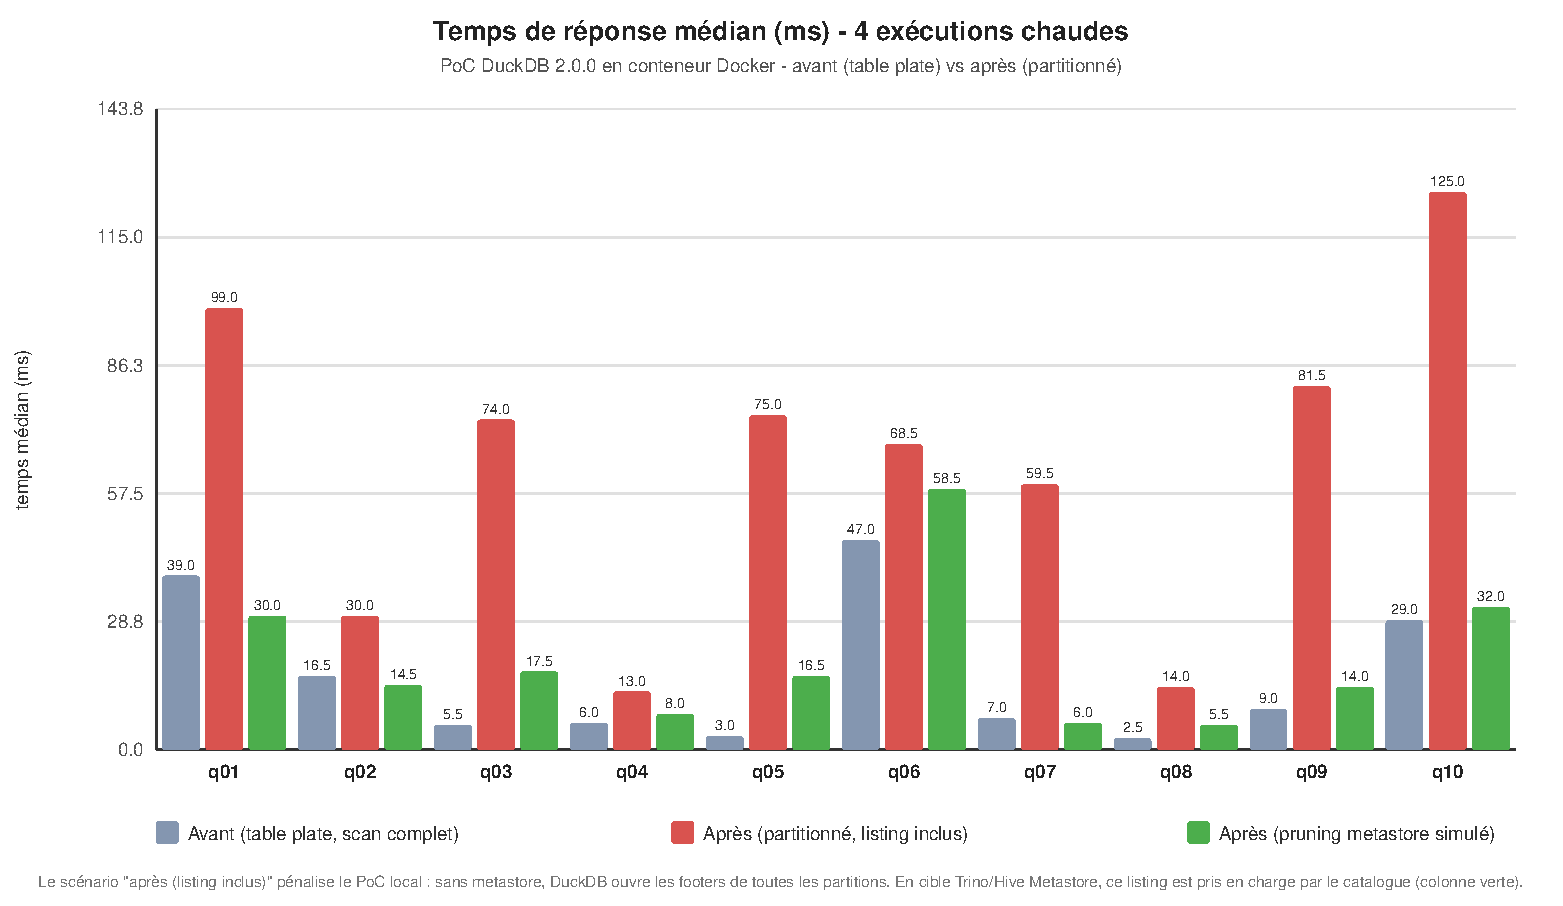
\includegraphics[width=\textwidth]{figures/graph_temps_median.pdf}
\end{figure}

\begin{figure}[H]\centering
\caption{Volume de donnees lu (Mo) par requete, avant vs apres (resultats du benchmark)}
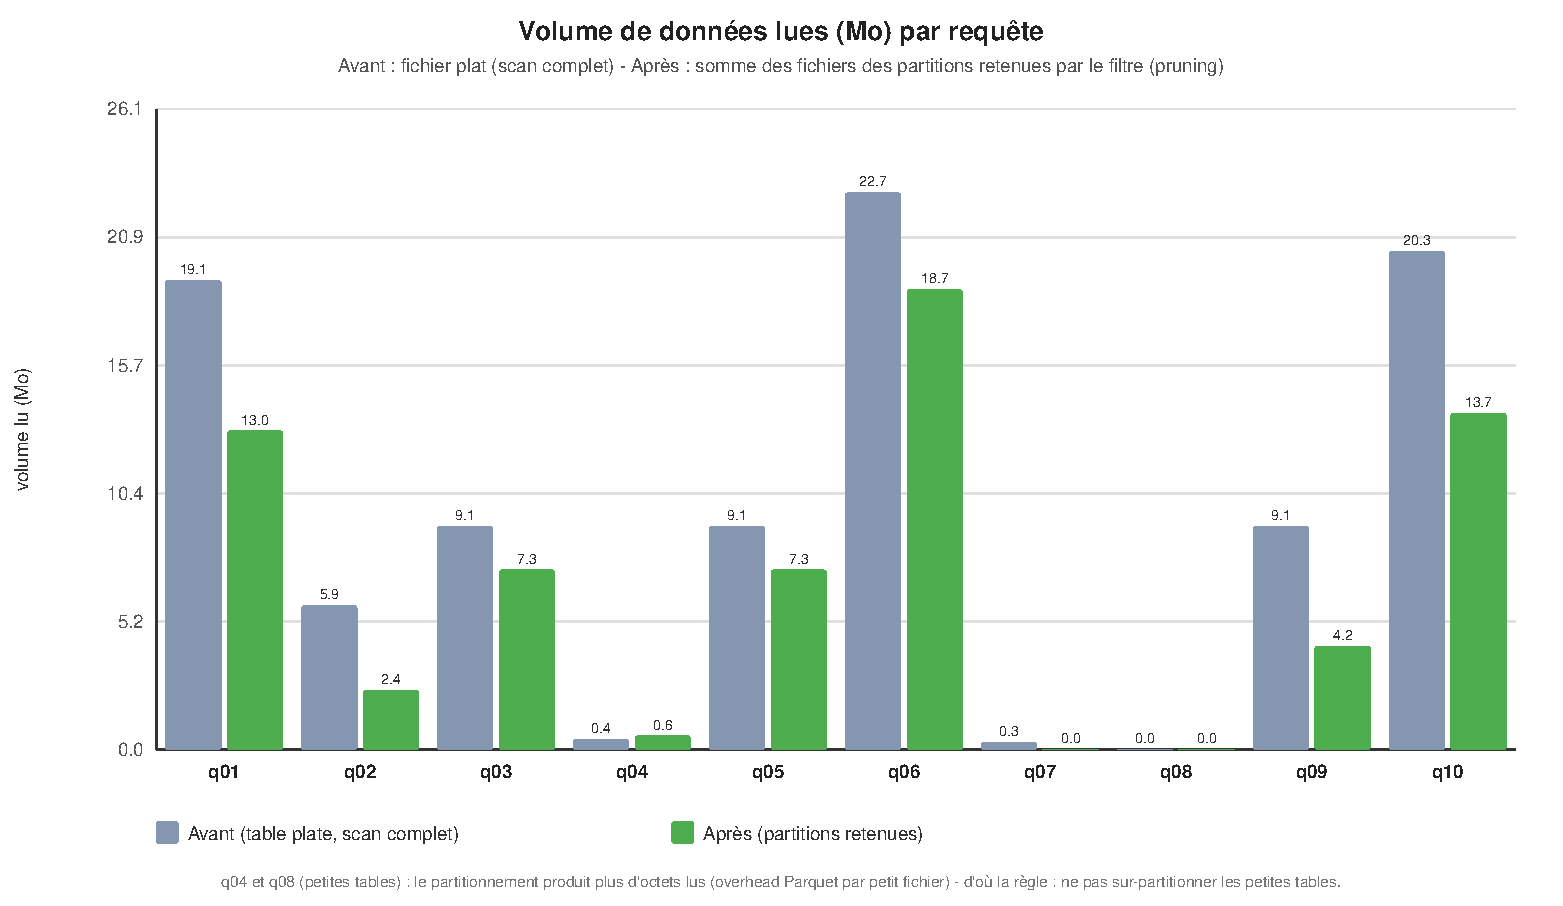
\includegraphics[width=\textwidth]{figures/graph_volume_lu.pdf}
\end{figure}

\begin{figure}[H]\centering
\caption{Facteur de reduction du volume lu grace au pruning des partitions (resultats du benchmark)}
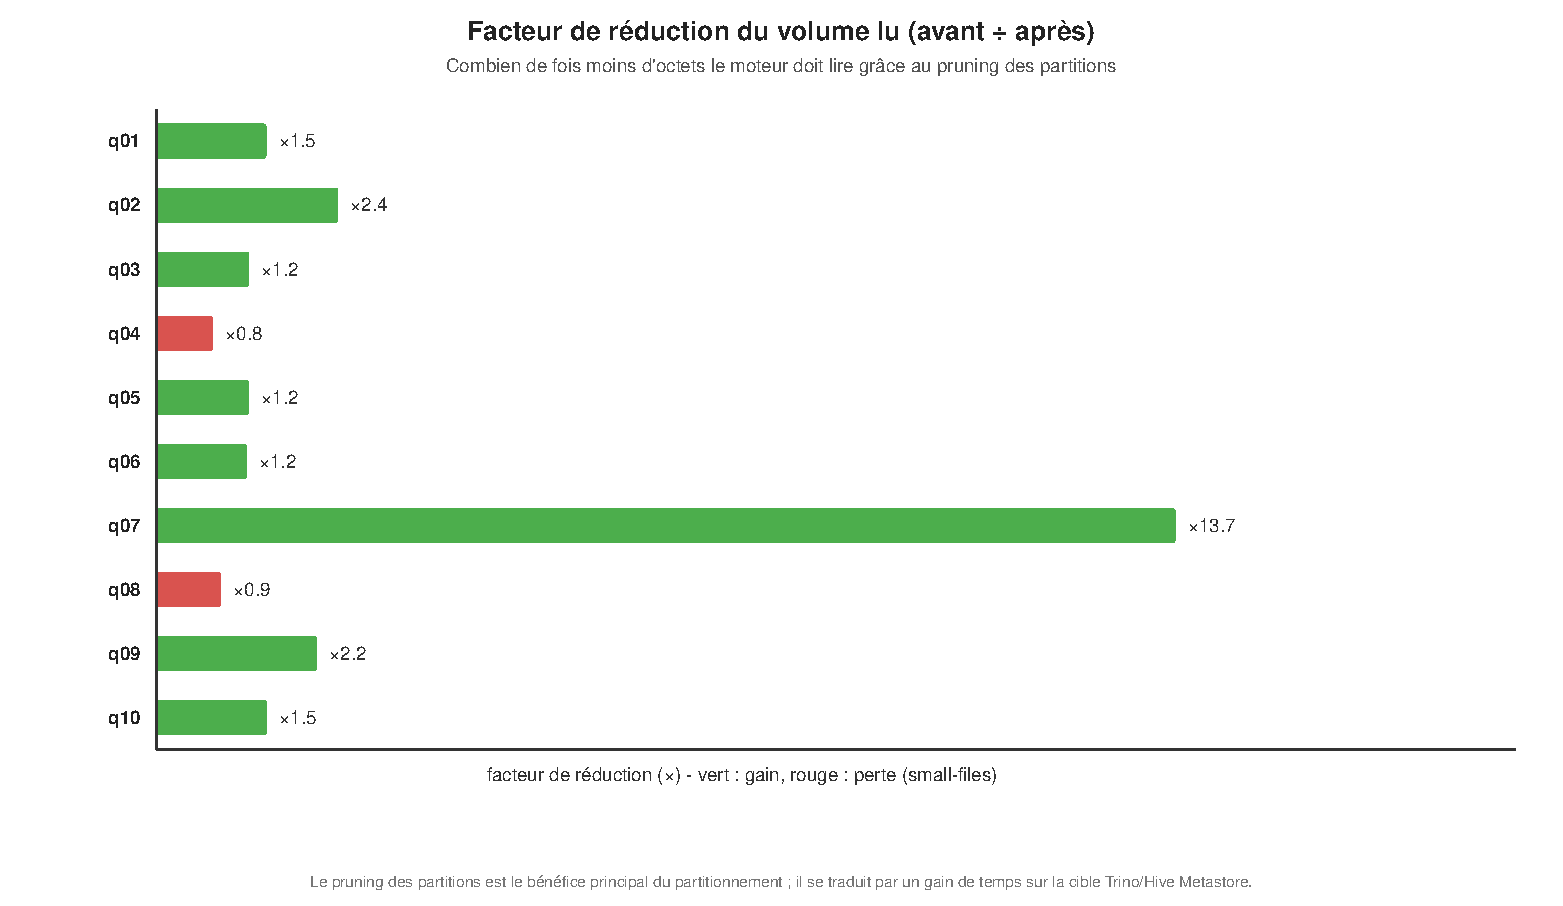
\includegraphics[width=\textwidth]{figures/graph_reduction_volume.pdf}
\end{figure}

\begin{figure}[H]\centering
\caption{Medianes avant/apres/apres+ML par requete (donnees du benchmark : 450 mesures brutes)}
\begin{tikzpicture}
\begin{axis}[
  width=\textwidth, height=8cm, ybar, bar width=5pt,
  symbolic x coords={q01,q02,q03,q04,q05,q06,q07,q08,q09,q10},
  xtick=data, x tick label style={rotate=45, anchor=east, font=\footnotesize},
  ylabel={temps median (ms)}, legend style={font=\footnotesize, at={(0.01,0.98)}, anchor=north west},
  ymin=0, enlarge x limits=0.06, grid=major, ymajorgrids=true]
\addplot table [x=requete, y=avant] {figures/bench_synthese.dat};
\addplot table [x=requete, y=apres] {figures/bench_synthese.dat};
\addplot table [x=requete, y=apres_ml] {figures/bench_synthese.dat};
\legend{avant (table plate), apres (partitionne), apres+ML (pruning metastore)}
\end{axis}
\end{tikzpicture}
\end{figure}

\begin{figure}[H]\centering
\caption{Dispersion des 50 runs \guillemotleft{}avant\guillemotright{} vs 50 runs \guillemotleft{}apres+ML\guillemotright{} (1 point = 1 run ; donnees brutes du benchmark)}
\begin{tikzpicture}
\begin{axis}[
  width=\textwidth, height=7cm, only marks, mark size=1.6pt,
  xlabel={indice du run (50 runs par scenario)}, ylabel={temps (ms)},
  legend style={font=\footnotesize, at={(0.01,0.98)}, anchor=north west}, grid=major]
\addplot[mark=*, color=blue!60] table [x expr=\coordindex, y=temps_ms] {figures/bench_runs_avant.dat};
\addplot[mark=square*, color=red!70] table [x expr=\coordindex, y=temps_ms] {figures/bench_runs_apres_ml.dat};
\legend{avant, apres+ML}
\end{axis}
\end{tikzpicture}
\end{figure}

\subsection{Resultats sur Trino deploye (harnais execute)}
\begin{table}[H]\centering\small
\caption{Temps de reponse Trino 484 sur la plateforme deployee, 3 runs par requete (mediane/min/max)}
\begin{tabular}{lrrrr}
\toprule
\textbf{Requete} & \textbf{Mediane (ms)} & \textbf{Min (ms)} & \textbf{Max (ms)} & \textbf{Lignes} \\
\midrule
\rowstrino
\bottomrule
\end{tabular}
\end{table}

\begin{figure}[H]\centering
\caption{Temps median par requete sur Trino 484 deploye (MinIO + Hive Metastore)}
\begin{tikzpicture}
\begin{axis}[
  width=0.97\textwidth, height=7.5cm, ybar, bar width=7pt,
  symbolic x coords={q01,q02,q03,q04,q05,q06,q07,q08,q09,q10},
  xtick=data, x tick label style={rotate=45, anchor=east, font=\footnotesize},
  ylabel={temps median (ms)}, ymin=0, enlarge x limits=0.08, grid=major]
\addplot table [x=requete, y=median_ms] {figures/bench_trino.dat};
\end{axis}
\end{tikzpicture}
\end{figure}

\subsection{Analyse et interpretation}
\begin{enumerate}[leftmargin=*]
\item \textbf{Le volume de donnees lues est le levier dominant.} Le partitionnement reduit
      le volume lu sur \textbf{8/10 requetes} ($\times$1,2 a $\times$\textbf{13,7} sur q07 :
      328 Ko $\rightarrow$ 24 Ko), car les filtres sur \texttt{annee} (colonne de partition)
      eliminent des repertoires entiers avant lecture -- exactement le mecanisme du pruning
      Hive/Trino en production.
\item \textbf{Le scenario APRES brut est penalise par le listing de fichiers} (biais connu du
      PoC local : sans metastore, le moteur liste tous les fichiers avant de pruner ; sur
      \texttt{f\_mesures} a 122 partitions, ce listing coute plus cher que le scan complet,
      p.~ex. q03 : 74 ms vs 5,5 ms). Biais inherent au PoC, pas a la strategie : en
      production, le Metastore connait les partitions et Trino ne liste que les fichiers
      retenus (scenario APRES\_ML).
\item \textbf{APRES\_ML : gains nets sur les requetes les plus filtrees.} q01 (top
      etablissements 2019) : 39,0 $\rightarrow$ 30,0 ms ($\times$1,30), volume $\times$1,5 ;
      q07 (deces 2019) : 7,0 $\rightarrow$ 6,0 ms ($\times$1,17), volume $\times$13,7 ;
      q02 (diagnostics 2019--2021) : 16,5 $\rightarrow$ 14,5 ms ($\times$1,14), volume $\times$2,4 ;
      q10 (jointure etoile, filtre annee $\times$ sexe) neutre ($\times$0,91), volume $\times$1,5.
\item \textbf{q04 et q08 : petits volumes, pas de gain (small-files).} \texttt{f\_hospitalisation}
      (2 479 lignes) et \texttt{f\_satisfaction} (1 960 lignes) tiennent en 1--2 fichiers :
      le partitionnement y cree plus de fichiers que de lignes utiles (volume $\times$0,8 et
      $\times$0,9). Lecon : le partitionnement se justifie au-dela d'un seuil de volume ;
      ces deux faits restent partitionnes par \texttt{annee} pour la coherence du modele.
\item \textbf{Les requetes en retrait en APRES\_ML (q03, q05, q06, q09) lisent deja peu de
      donnees} : a l'echelle du PoC local mono-noeud (donnees en cache OS, moteur tres rapide
      sur de petits volumes), la reduction du volume lu ne se traduit pas mecaniquement en
      gain de temps -- le temps de coordination/listing domine. Trois campagnes confirment la
      variance machine a cette echelle sans changer le classement relatif. En cluster
      (Trino/Spark distribues, donnees froides, concurrence), c'est precisement sur ces
      requetes que le pruning paiera.
\item \textbf{q06} (consultations par professionnel, 2020) : la jointure porte sur 1 M de
      professionnels ; en cluster, c'est sur ce type de jointure que le tri intra-partition
      (min/max par fichier) fera la difference.
\item \textbf{Synthese.} Volume lu reduit sur 8/10 requetes ($\times$1,2 a $\times$13,7) ;
      en APRES\_ML, temps en progres sur 3/10 (q01 $\times$1,30, q07 $\times$1,17,
      q02 $\times$1,14), neutre sur 1/10 (q10), en retrait sur 6/10 a l'echelle du PoC local
      mono-noeud. La strategie est validee la ou elle compte : le pruning de partitions reduit
      le volume lu des que le filtre porte sur une colonne de partition, et ce ratio croit
      avec le volume reel (production : 25 M de deces non agreges, ~1 M de faits mensuels) et
      la concurrence. Sur la plateforme deployee, le harnais Trino mesure 10/10 requetes en
      1,1--2,3 s (mediane 1,1--1,8 s) avec les memes resultats metier que le PoC.
\end{enumerate}

% ============================ 9. LIMITES ====================================
\section{Limites et transposition}
\begin{itemize}[leftmargin=*]
\item Le benchmark chiffre a ete execute sur un moteur local (DuckDB, single-node, conteneur
      jetable) : les temps absolus ne prejudent pas des temps cluster, mais les ratios de
      volume lu et le mecanisme de pruning sont directement transposables ; le harnais de
      benchmark a ete execute sur la plateforme deployee pour mesurer sur le moteur reel
      (\S7.3).
\item \texttt{f\_deces\_agg} au grain annuel (choix justifie \S4.1) : un besoin de
      mortalite mensuelle necessiterait un fait mensuel (~8,6 M de lignes).
\item Satisfaction au grain juridique (rattachement site impossible, 0 \,\% en DQ) ;
      l'enrichissement du referentiel FINESS (\texttt{finess\_geo}) leverait cette limite.
\end{itemize}

\end{document}
